%%                       Template LaTeX pour SSTIC
%% 
%% 
%% Utilisation
%% ===========
%% 
%% Pour compiler les sources, c'est aussi simple que :
%%     $ make
%% 
%% Le résultat est dans sstic-actes.pdf
%% 
%% Ce modèle doit être la base commune à tous les articles LaTeX pour
%% SSTIC.
%% 
%% Un exemple d'article est disponible dans le répertoire MonNom/ En
%% tant qu'auteur, vous devez copier ce répertoire et l'adapter.
%% 
%% Important : Vous ne devez pas pas toucher aux fichiers préfixés par _
%% 

\documentclass[b5paper,11pt]{llncs}

%% Nous avons déjà sélectionné quelques packages, si vous avez besoin
%% d'ajouter un nouveau package, veuillez contacter l'équipe (actes
%% (AT) lists.sstic.org) car nous devons vérifier la compatibilité des
%% modules entre eux.
%% 

\usepackage[french]{babel}
\usepackage[utf8x]{inputenc}
\usepackage[fit]{truncate}
\usepackage{xspace}
\usepackage{xcolor}
\usepackage{graphicx}
\usepackage{fancyhdr}
\usepackage{listings}
\usepackage{ifthen}
\usepackage{url}

\usepackage{makeidx}
\makeindex

\usepackage[T1]{fontenc}
\usepackage{tabularx}
\usepackage{array}
\usepackage{multirow}
\usepackage{lscape}

\renewcommand\andname{et}
\renewcommand\lastandname{ et}

\newcommand{\xxx}{{\bf \LARGE \textcolor{red}{XXX}}\xspace}
\newcommand{\XXX}{\xxx}
\newtheorem{exx}{Exemple}

\def\keywordname{{\bf Mots-cl\'es:}}
\def\ackname{Remerciements.}
\def\andname{et}
\newcommand{\keywords}[1]{\par\addvspace\baselineskip\noindent\keywordname\enspace\ignorespaces#1}


\definecolor{grigri}{RGB}{233,232,234}
\lstset{breaklines=true,
        tabsize=4,
        boxpos=c,
        showstringspaces=false,
        basicstyle=\ttfamily\scriptsize,
        aboveskip=\bigskipamount,
        belowskip=\bigskipamount,
        captionpos=b,
        language=C,
        extendedchars=false
        basicstyle=\scriptsize\sffamily\color{darkgray},
        keywordstyle=\bfseries\color{purple},
        identifierstyle=\bfseries\color{black},
        commentstyle=\ttfamily\itshape\color{purple},
        stringstyle=\ttfamily\color{brown},
        showstringspaces=false,
        frame=leftline,
        backgroundcolor=\color{grigri},
        fillcolor=\color{grigri}}

\lstloadlanguages{[Sharp]C,[x86masm]Assembler,java,PHP,C,Python}

%%%%%%%%%%%%%%%%%%%%%%%%%%%%%%%%%%%%%%%%%%%%%%%%%%%%%%%%%%%%%%%%%%%%%%%%%%%%%%%%

% example d'usage:
%     \settitle[Mon titre court]{Mon titre super mégalong de la mort}
\newcommand{\theshorttitle}{}
\newcommand\settitle[2][]{%
 \title{#2}%
 \ifthenelse{\equal{#1}{}}%
  {\renewcommand{\theshorttitle}{#2}\toctitle{#2}\titlerunning{#2}}%
  {\renewcommand{\theshorttitle}{#1}\toctitle{#1}\titlerunning{#1}}%
}

\newcommand{\theshortauthor}{}
\newcommand\setauthor[2][]{%
 \author{#2}%
 \ifthenelse{\equal{#1}{}}%
  {\renewcommand{\theshortauthor}{#2}\tocauthor{#2}\authorrunning{#2}}%
  {\renewcommand{\theshortauthor}{#1}\tocauthor{#1}\authorrunning{#1}}%
}

\pagestyle{fancy}
\fancyhf{}
\setlength{\headheight}{16pt}
\fancyhead[LE,RO]{\thepage}
\fancyhead[RE]{\truncate{.90\headwidth}{\theshorttitle}}
\fancyhead[LO]{\theshortauthor}

\newcommand\myclearpage{\thispagestyle{empty}}

%%%%%%%%%%%%%%%%%%%%%%%%%%%%%%%%%%%%%%%%%%%%%%%%%%%%%%%%%%%%%%%%%%%%%%%%%%%%%%%%

\bibliographystyle{plain}

\sloppy

\begin{document}

%\frontmatter

%\settitle[CorkaMIX]{Polyglottes binaires et implications}

\newcommand{\TODO}[1]{}
%\newcommand{\TODO}[1]{\textcolor{red}{TODO:~#1}}

\newcommand{\WIN}[0]{\emph{Windows}\xspace}

\newcommand{\ZIP}[0]{\emph{ZIP}\xspace}
\newcommand{\JAVA}[0]{\emph{Java}\xspace}
\newcommand{\GIF}[0]{\emph{GIF}\xspace}
\newcommand{\PE}[0]{\emph{PE}\xspace}
\newcommand{\ELF}[0]{\emph{ELF}\xspace}
\newcommand{\MACHO}[0]{\emph{Mach-O}\xspace}
\newcommand{\JAR}[0]{\emph{JAR}\xspace}
\newcommand{\HTML}[0]{\emph{HTML}\xspace}
\newcommand{\PDF}[0]{\emph{PDF}\xspace}

\setauthor[Ange~Albertini]{Ange Albertini\\
  \email{ange.albertini@gmail.com}}
\institute{Corkami.com}


\maketitle

\begin{abstract}
De l'exploitation à l'infection, les {\it malwares} modernes utilisent de nombreux formats de fichier binaires.
Il est crucial de pouvoir correctement les identifier et les analyser, si possible de manière automatique.
Bien que ces formats soient a priori clairement différenciés, il est parfois possible de combiner certains d'entre eux dans un seul et même fichier.
On parle alors de fichiers {\it polyglottes}.
De tels fichiers {\it polyglottes} ont donc dans un premier temps été créés.
Ensuite, plusieurs caractéristiques non documentées de chaque format concerné ont été rajoutées, pour mettre en évidence l'importance du problème entre les limites des documentations officielles, et la réalité (du monde des virus).
Les conséquences sur le fonctionnement des outils de sécurité sont finalement mises en évidence, avec ce que ça implique pour l'utilisateur final.
\end{abstract}


\section{Introduction}

\subsection{État de l'art}

Un fichier polyglotte est un fichier qui peut être interprété dans plusieurs langages différents.  Un des plus simple d'entre eux, représenté par le Polyglot de David Kendall dans le listing~\ref{lst:albertini:polyglot}, fonctionne en Ruby, Perl, PHP, ksh, Scheme, Lisp, Clojure, Plan. Les {\it polyglottes} peuvent aller beaucoup plus loin, jouant sur les différences d'interprétation et de {\it pré-processing} de chaque langage inclus dans le fichier.


\begin{lstlisting}[language={},caption={Un programme polyglotte simple.},label={lst:albertini:polyglot}]
 (print "Hello, world!\n");
\end{lstlisting}

La première utilisation de fichiers polyglottes dans le monde des virus est GIFAR~\cite{albertini:wikipedia:gifar}~:

un GIFAR résulte de l'ajout d'une classe \JAVA stockée au format \JAR à la suite d'une image au format \GIF. En effet, le \GIF est un format d'image couramment utilisé sur le Web, notamment pour les avatars dans les forums de discussion. Une fois le fichier sur le serveur, il est ensuite utilisable aussi comme une classe \JAVA. Si on utilise cette classe dans un script quelconque sur le serveur, le navigateur laissera accèder à la classe, même si elle est malveillante, car elle est maintenant hébergée sur le même site.

Julia Wolf~\cite{albertini:wolf:omgwtfpdf} a introduit le concept de \ZIP et \emph{Portable Document Format} --- dit \PDF --- combinés, ce qui permet de tromper les outils de sécurité et ainsi permettre d'exfiltrer des informations, ou passer pour un fichier innocent.

Jonas Magazinius~\cite{albertini:magazinius:polyglots} s'est également penché sur la question, en combinant notamment image \emph{JPG} et document \PDF.

En revanche, les formats de fichiers binaires sont, eux, rarement compatibles, car exclusifs: en effet, la majeure partie d'entre eux doivent nécessairement débuter par un marqueur (on parle aussi de \emph{magic number} en anglais), spécifique à chaque format, à de rares exceptions près (tel {\tt 0xcafebabe}, pour le format \MACHO universel et les classes \JAVA).

Il ne semble donc pas possible de combiner des formats binaires en général. Cependant, il y a quelques exceptions:
\begin {itemize}
\item tout d'abord, certains formats de fichier n'ont aucun en-tête, tels que le \emph{Master Boot Record} --- dit \emph{MBR} --- ou les fichiers \emph{COMMAND FILE} --- dit \emph{COM}. Il est donc possible de créer un secteur de démarrage à la fois au format \emph{GRUB} et au format \emph{MBR}~\cite{albertini:scott:metalkiller}, ou bien un fichier \emph{COM} qui soit également un fichier exécutable linux \ELF.

\item d'autre parts, d'autre formats de fichiers n'imposent pas que le marqueur soit présent au début du fichier: c'est le cas des archives (\ZIP, \emph{RAR}\ldots), des pages \HTML, et des documents \PDF.

\item enfin, certains formats, bien que commencant obligatoirement au premier déplacement, autorisent un grand espace entièrement modifiable juste après la signature, tels que le format d'exécutable \emph{Portable Executable} --- dit \PE --- et le format d'image \emph{PICT}.
\end{itemize}

Hélas, certains formats utilisables à des fins malveillantes sont librement combinables dans un seul et même fichier, mais de plus, il s'agit des formats parmi les plus utilisés ces dernières années pour la prolifération de {\it malware}:
en effet, la chaîne d'infection complète par un virus la plus répandue est une page \HTML, contenant du Javascript, qui va charger un fichier \JAVA profitant d'une vulnérabilité, qui lui-même va télécharger le virus final, sous forme d'un exécutable \WIN, au format \emph{PE} --- et on peut effectivement combiner une page \HTML, une classe \JAVA, et un fichier binaire au format \PE.

Un autre vecteur d'infection répandu est un \PDF activant une vulnérabilité, dont le \emph{shellcode} téléchargera un \PE. Et là encore, \PE et \PDF sont combinables dans un seul et même fichier.

\subsection{Pivot}

Le format pivot de la grande majeure partie des virus est le format de binaire universel de \WIN, le format \PE. Pour ce rôle unique dans la chaîne virale, il a donc été choisi comme point de départ.

\section{Exploration du format \PE}
Ce format stipule que le fichier commence par une structure \texttt{IMAGE\_DOS\_HEADER}, de \texttt{0x40} octets:
\begin{itemize}
\item les 2 premiers octets de cette structure définissent un champ appelé \texttt{e\_magic}, qui contient obligatoirement la signature \texttt{MZ}~: Il est donc impossible de le combiner à tout autre format imposant une signature spécifique au déplacement 0.
\item tous les champs suivants, à l'exception du dernier, ne concernent que la fonctionnalité \emph{DOS} de l'exécutable --- qui se borne en majeure partie à afficher un message d'erreur. Elle est totalement ignorée quand le fichier est chargé en tant que \PE.
\item le dernier champ, \texttt{e\_lfanew}, est un pointeur sur 32 bits vers la structure suivante de l'exécutable.
\end{itemize}

On sait donc que notre fichier doit commencer par {\tt M} et {\tt Z}, et qu'au déplacement \texttt{0x3C} doit se trouver un pointeur. Entre les deux, on peut y faire ce que l'on veut, tout en gardant la fonctionalité \PE intacte. On peut même mettre l'en-tête \PE à la fin du fichier sans problème.

\subsection{Création d'une page \HTML dans un exécutable}

Le laxisme omniprésent dans les pages \HTML fait qu'au final, les navigateurs se contentent d'ignorer un peu tout --- quand bien même ce serait de l'information non encodable en \emph{ASCII} --- au cas où un tag \texttt{<HTML>} finirait par être présent.

Ainsi, le simple fait de rajouter à la fin d'un exécutable du code \HTML va en faire une page web fonctionnelle, pour peu qu'on renomme l'extension du fichier, comme le montre la figure~\ref{fig:albertini:htmlnotepad}.

\begin{figure}[ht]
  \centering
  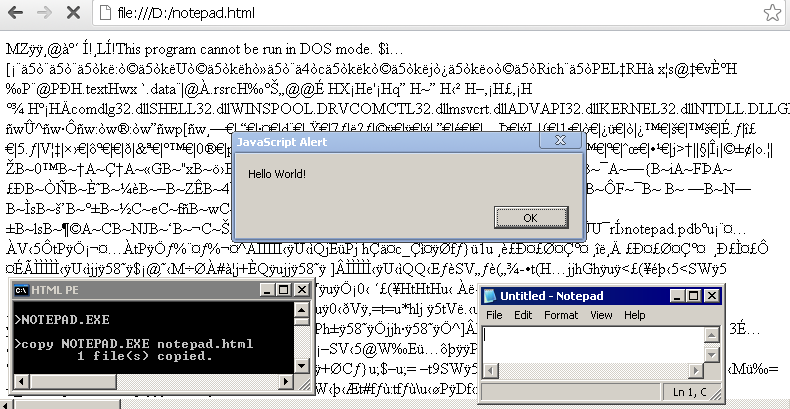
\includegraphics[width=0.8\textwidth]{albertini/img/htmlnotepad}
  \caption{Le bloc-note \WIN avec une page HTML ajoutée à la fin.}
  \label{fig:albertini:htmlnotepad}
\end{figure}

Cela dit, bien que le fichier soit fonctionnel dans les deux formats, les données binaires perturbent l'affichage de la page web, bien que celles-ci soient placées avant le tag ouvrant \texttt{<HTML>}.
On va donc jouer sur les \emph{Cascaded Style Sheet} pour effacer ces données et ainsi avoir un résultat visuellement parfait. Ou sinon, on peut insérer ce tag juste après la signature du \PE, auquel cas on aura juste un \texttt{MZ} affiché sur la page.

De même, si on souhaite rajouter quelque chose après la page web et son script, il nous suffit d'ouvrir un bloc de commentaire non fermé \texttt{<!----}.

À noter que si une page web doit avoir une extension précise pour être visualisée correctement, un exécutable \WIN n'a besoin d'aucune extension particulière pour être exécuté via les APIs \WIN.

\subsection{Concaténation d'un \PDF et d'un exécutable}

La spécification officielle stipule que la première ligne d'un \PDF doit être sa signature:
\begin{center}
  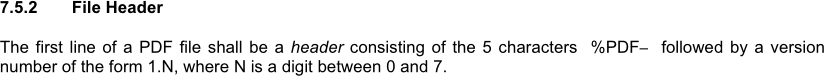
\includegraphics[width=0.8\textwidth]{albertini/img/pdfsigtheory}
\end{center}

En pratique, il n'en n'est rien, il est juste requis sous \emph{Adobe Reader} qu'une signature valide soit présente dans les 1024 (\texttt{0x400}) premiers octets.

\begin{figure}[ht]
  \centering
  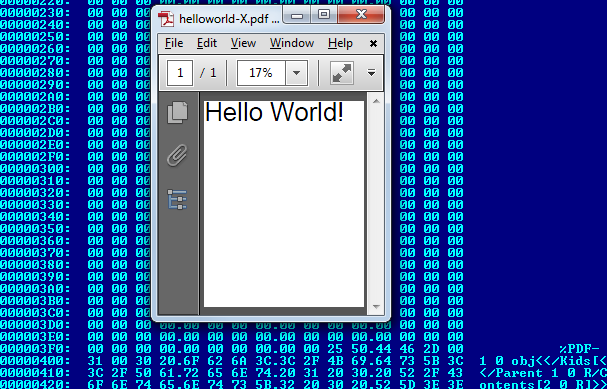
\includegraphics[width=0.8\textwidth]{albertini/img/pdfsigpractice}
  \caption{Un \PDF dont la signature est à la fin des \texttt{1024} premiers octets est toujours reconnu par \emph{Adobe Reader}.}
  \label{fig:albertini:pdfsigpractice}
\end{figure}

On peut donc, dans un premier temps, rajouter à la fin d'un petit exécutable un \PDF dans son intégralité, et les deux fonctionneront encore comme on s'y attend, comme dans la figure~\ref{fig:albertini:tinyPEPDF}.

\begin{figure}[ht]
  \centering
  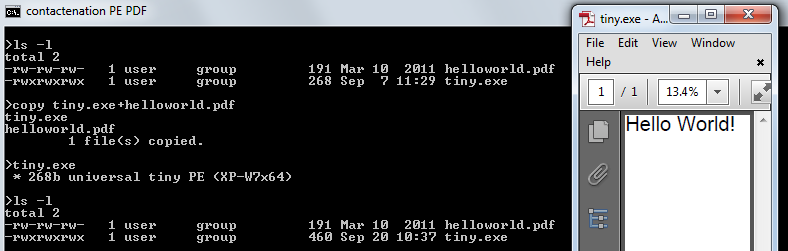
\includegraphics[width=0.8\textwidth]{albertini/img/tinyPEPDF}
  \caption{Un \PDF greffé à la fin d'un petit exécutable \PE.}
  \label{fig:albertini:tinyPEPDF}
\end{figure}

Dans le cas d'un \PE plus gros que \texttt{1024} octets, on devra rajouter la signature \PDF dans l'en-tête \PE.

Il arrive cependant que le \PE, stocké au format binaire, contienne des séquences de caractères qui seront interprétées par la visionneuse \PDF. Pour cela, il suffit d'entourer le reste du \PE d'une structure d'objet \emph{stream} fictive, et ainsi son contenu ne sera pas analysé, puisqu'il n'est pas référencé dans la hiérarchie du document, comme dans la figure~\ref{fig:albertini:pdfnotepad}.

\begin{figure}[ht]
  \centering
  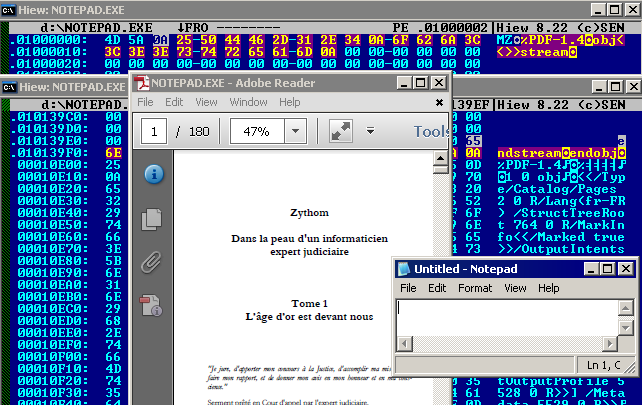
\includegraphics[width=0.8\textwidth]{albertini/img/pdfnotepad}
  \caption{Le bloc-note \WIN avec un fichier \PDF ajouté à la fin.}
  \label{fig:albertini:pdfnotepad}
\end{figure}


\subsection{Une archive \ZIP dans un exécutable}
Le format \ZIP n'impose rien quant au début du fichier --- il est lu en partant de la fin, et tolère des données avant ou après la structure du format elle-même. Un fichier \ZIP peut donc se trouver n'importe où dans un autre fichier.

Une classe \JAVA peut être exécutée directement, ou en étant contenue dans un fichier {\em Java Archive}, dit \JAR.
Un fichier \JAR n'est qu'une archive \ZIP contenant une ou plusieurs classes \JAVA, et un fichier texte (\texttt{manifest}) au contenu bien défini.

Contrairement à un \ZIP standard, un fichier \JAR doit terminer strictement le fichier: si on rajoute ne serait-ce qu'un seul octet à la suite, \JAVA ne reconnaît plus ce fichier comme valide.

\subsection{Récapitulons}

À l'aide des manipulations décrites précédemment, nous obtenons donc:
\begin{enumerate}
\item le début d'un \PE
\item une signature \PDF dans ses \texttt{1024 - 6} premier octets
\item la suite du \PE, inclue dans un objet \texttt{stream} \PDF
\item dans un ordre quelconque~:
\begin{itemize}
\item le reste du \PDF, finissant l'objet fictif
\item la page \HTML
\end{itemize}
\item un \ZIP, optionnellement un \JAR
\end{enumerate}

\section{Détails de mise en oeuvre}

Un simple fichier polyglotte est donc faisable via des opérations de concaténations et quelques modifications manuelles.

Pour pousser l'expérience quant au comportements d'outils de sécurité, des propriétés anormales seront ajoutées aux formats inclus, dans le but de tester leur robustesse.

Afin d'y arriver, l'intégralité du fichier sera faite à la main, pour en garder le contrôle complet.

Toutes les structures sont crées à partir de zéro, en assembleur: en effet, un assembleur standard a la possibilité de définir chaque octet manuellement, et aussi de créer des fonctions et des structures, qui vont faciliter la création du fichier, tout en gardant le contrôle de chaque octet.

Quand un fichier est stocké dans une archive \ZIP sans compression, il est stocké dans son intégralité, à l'identique: inclure un fichier dans une archive ne revient donc qu'à ajouter en-tête et pied de page.

\subsection{Un \PE fait main}

\subsubsection*{Peu d'éléments définis}

Notre exécutable contient \texttt{Hello World} compilé en assembleur standard, mais seulement 18 éléments sont absolument indispensables, toutes structures confondues, tel que le montre la figure~\ref{fig:albertini:empty_pe_header}.

\begin{figure}[ht]
  \centering
  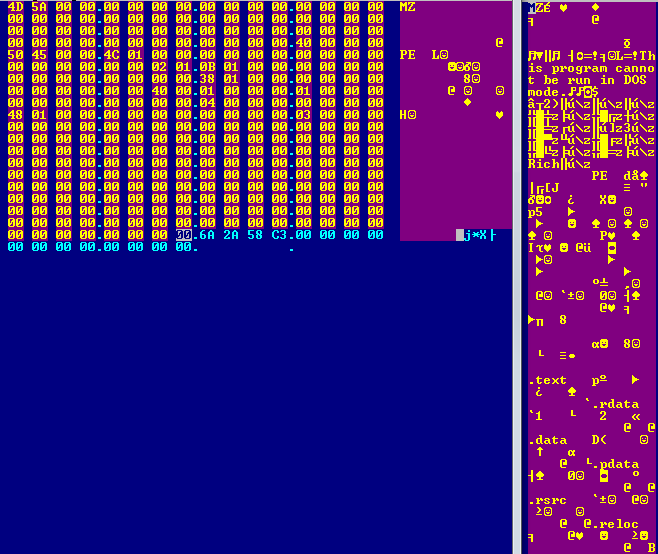
\includegraphics[width=0.8\textwidth]{albertini/img/empty_pe_header}
  \caption{Comparaison d'en-têtes \PE.}
  \label{fig:albertini:empty_pe_header}
\end{figure}

On obtient donc un \PE qui va faire échouer les outils naïfs qui déterminent la validité du fichier d'après des éléments non indispensables.

\subsubsection*{Pas de sections}

Quand un exécutable utilise des alignements faibles, tout l'exécutable est chargé en mémoire indépendamment de la table des sections. Il devient dans ce cas possible de ne définir aucune section (\emph{NumberOfSections = 0}), et de ne pas avoir de table de section (\emph{SizeOfOptionalHeader = 0}).

Là encore, il fera échouer les outils qui analysent ce format section par section.

\subsubsection*{Utilisation d'instructions non documentées}

Un outil de sécurité avancé va essayer d'émuler l'exécution du début du fichier, pour déterminer s'il est malveillant ou non.

Certaines instructions, non documentées, peuvent amener un tel émulateur à abandonner, car il ne peut déterminer comment procéder. La présence de telles instructions ne peut vraisemblablement pas amener à qualifier le fichier de malveillant, car il pourrait s'agir de nouvelles instructions d'un processeur récent.

Certaines de ces instructions comme {\tt SetALC} ou les {\tt nop} multi-octets sont absentes de la documentation Intel (figures~\ref{fig:albertini:undoc_setalc} et \ref{fig:albertini:undoc_nop}), mais présentes dans la documentation AMD (figures~\ref{fig:albertini:salc_amd} et \ref{fig:albertini:nop_amd}), parfois uniquement sous le status \emph{réservé}.


Ces instructions ne sont reconnues dans aucun outil Microsoft (figure~\ref{fig:albertini:corkamix_windbg}), car ils suivent la documentation Intel à la lettre.


\begin{figure}[ht]
  \centering
  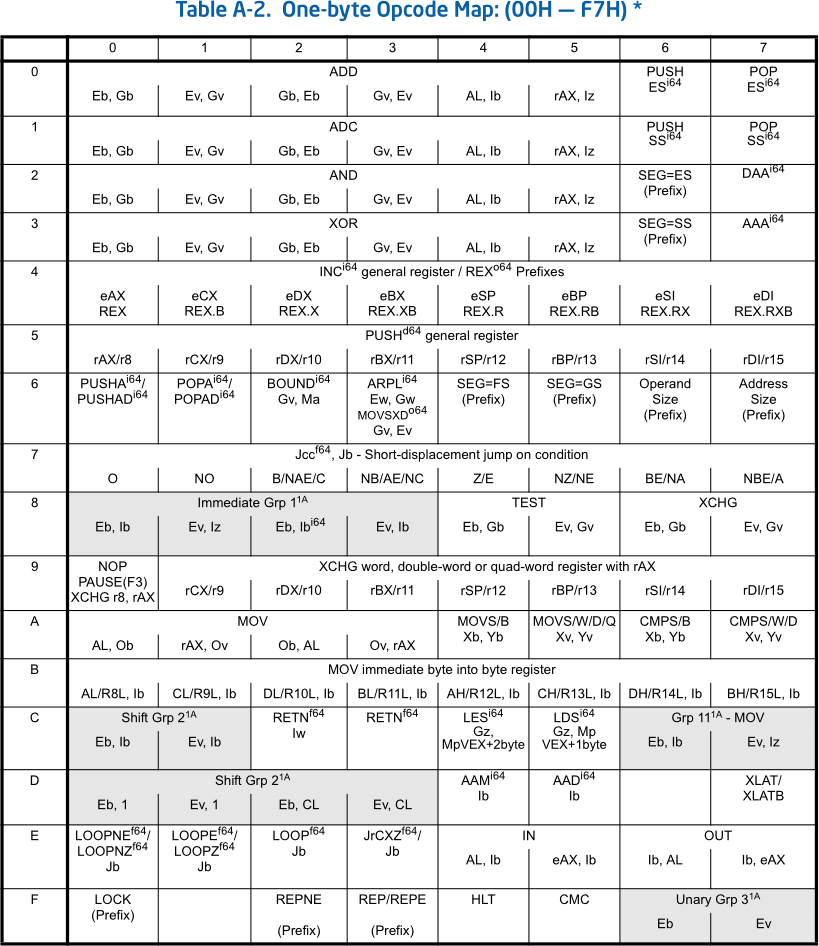
\includegraphics[width=0.8\textwidth]{albertini/img/undoc_setalc}
  \caption{La documentation officielle n'indique rien pour l'octet \texttt{D6}.}
  \label{fig:albertini:undoc_setalc}
\end{figure}

\begin{figure}[ht]
  \centering
  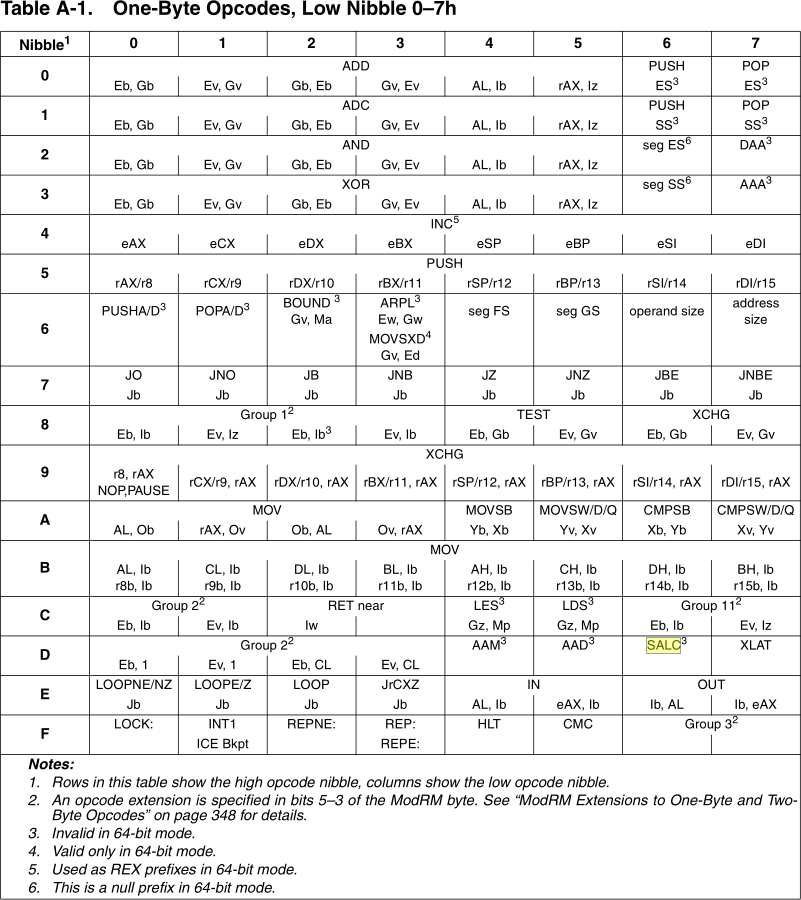
\includegraphics[width=0.8\textwidth]{albertini/img/salc_amd}
  \caption{SetALC est documenté par AMD.}
  \label{fig:albertini:salc_amd}
\end{figure}

\begin{figure}[ht]
  \centering
  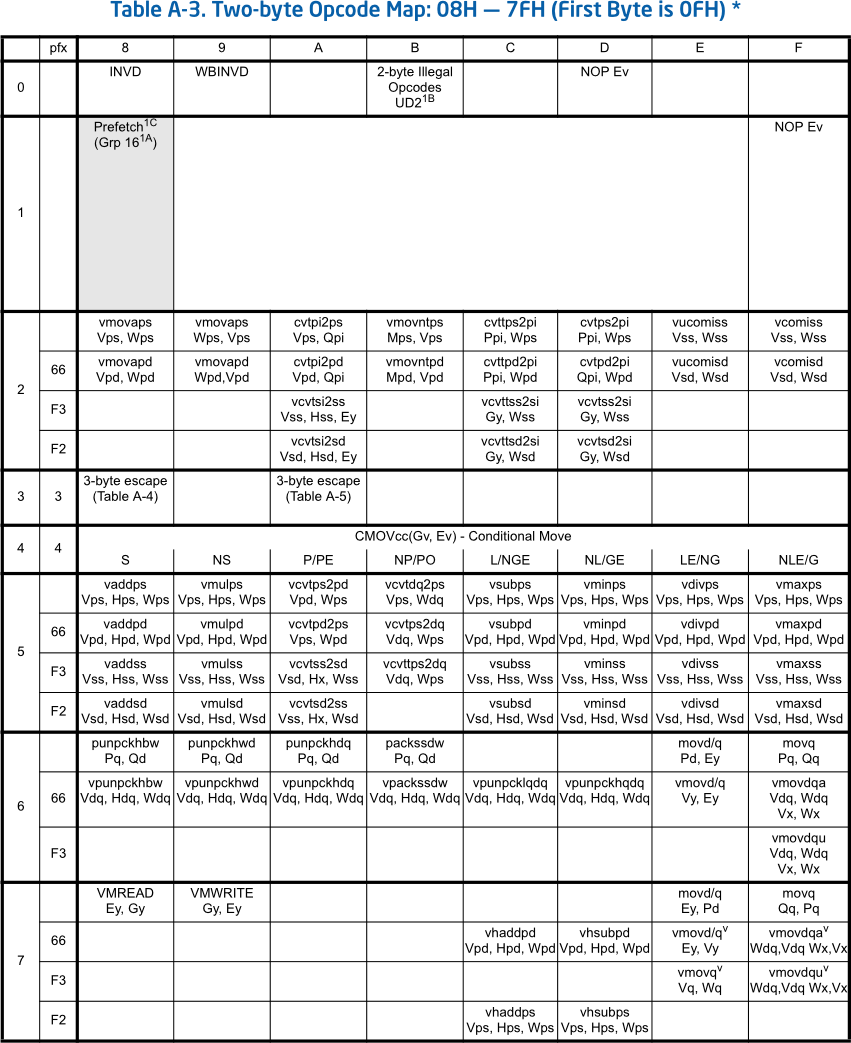
\includegraphics[width=0.8\textwidth]{albertini/img/undoc_nop}
  \caption{La documentation Intel ne mentionne NOP que pour les octets \texttt{0F 1F}.}
  \label{fig:albertini:undoc_nop}
\end{figure}

\begin{figure}[ht]
  \centering
  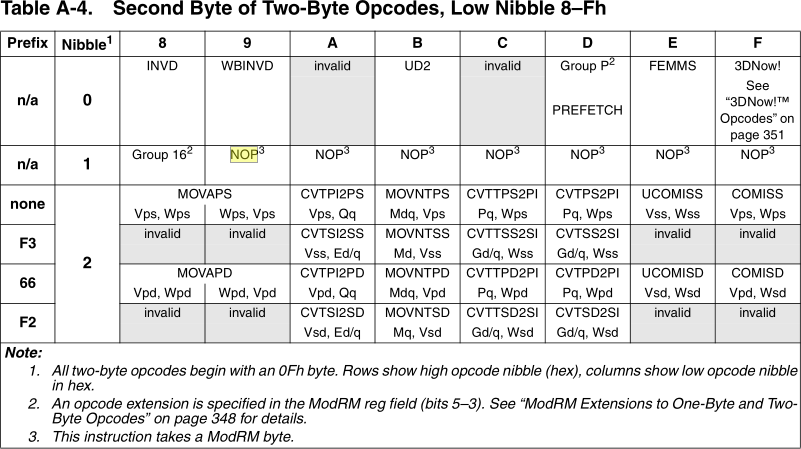
\includegraphics[width=0.8\textwidth]{albertini/img/nop_amd}
  \caption{Le NOP de plusieurs octets est complètement documenté par AMD.}
  \label{fig:albertini:nop_amd}
\end{figure}

\begin{figure}[p]
  \centering
  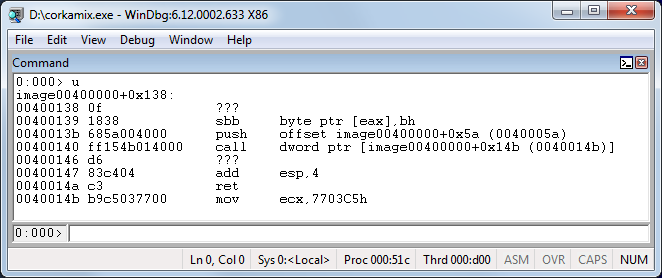
\includegraphics[width=0.8\textwidth]{albertini/img/corkamix_windbg}
  \caption{WinDbg montre plusieurs instructions inconnues.}
  \label{fig:albertini:corkamix_windbg}
\end{figure}

Pour implémenter ces instructions, on doit générer certaines à la main, un assembleur standard ne les gérant pas forcément.

\subsubsection*{Une structure d'import très compacte}

le \emph{DataDirectory} des imports pointe vers une liste de \emph{descripteurs}.
Cette liste se termine en théorie par un descripteur entièrement nul, mais en réalité uniquement si ses champs \texttt{Name} ou \texttt{FirstThunk} sont nuls.

La table des adresses, si elle est suffisamment petite, peut-être intégrée dans un des descripteurs, alors qu'elle utilise habituellement son propre espace du fichier.

De même, le nom de la DLL, même amputé de son extension, peut être inclus dans un des descripteurs, ainsi que la structure \texttt{IMAGE\_IMPORT\_BY\_NAME} de l'import, alors qu'eux aussi sont censés être instanciés séparément, hors des descripteurs.

On obtient donc une table d'import très compacte, avec beaucoup d'irrégularités, mais pourtant 100~\% gérée et fonctionnelle (figure~\ref{fig:albertini:imports}) par \WIN.

\begin{figure}[p]
  \centering
  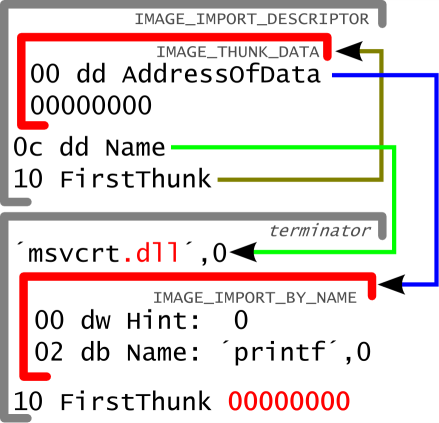
\includegraphics[width=0.5\textwidth]{albertini/img/imports}
  \caption{Une structure d'imports avec beaucoup de malformations.}
  \label{fig:albertini:imports}
\end{figure}

Ces astuces font que les outils les plus avancés échouent à analyser le \PE parfaitement. Notamment, à l'heure de création de ces recherches, la dernière version de Hiew et IDA échouent à les gérer (figure~\ref{fig:albertini:imports_error}).

\begin{figure}[p]
  \centering
  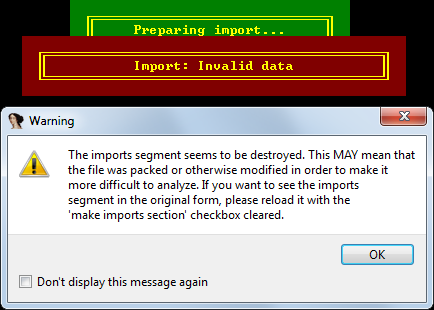
\includegraphics[width=0.5\textwidth]{albertini/img/imports_error}
  \caption{Une structure d'imports non gérée par Hiew ou IDA.}
  \label{fig:albertini:imports_error}
\end{figure}



\subsection{Un \PDF très compact}
La signature \PDF, bien qu'officiellement \texttt{\%PDF-1.?}, peut en fait être tronquée, selon la visionneuse employée.

La signature de fin \texttt{\%\%EOF} est absolument superflue, ansi que toute référence à une longueur dans les objets \texttt{stream}.

De même, la table \texttt{xref} est supprimable, ansi que les terminateurs d'objet \texttt{endobj}.

Enfin, le trailer final est réduit à son strict minimum.

On obtient donc, dans des cas extrêmes, un fichier \PDF particulièrement réduit de 36 octets fonctionnant sous Adobe Reader (listing~\ref{lst:albertini:tinypdf}).

\begin{lstlisting}[language={},caption={Un \PDF valide de 36 octets.},label={lst:albertini:tinypdf}]
%PDF- trailer<</Root<</Pages<<>>>>>>
\end{lstlisting}

\subsection{Un \emph{patchwork} binaire}

Au final, on obtient un fichier fonctionnel dans tous les formats inclus (figure~\ref{fig:albertini:corkamix}), et de nombreuses caractéristiques non documentées, qui font échouer des outils d'analyse et des anti-virus répandus.

\begin{figure}[p]
  \centering
  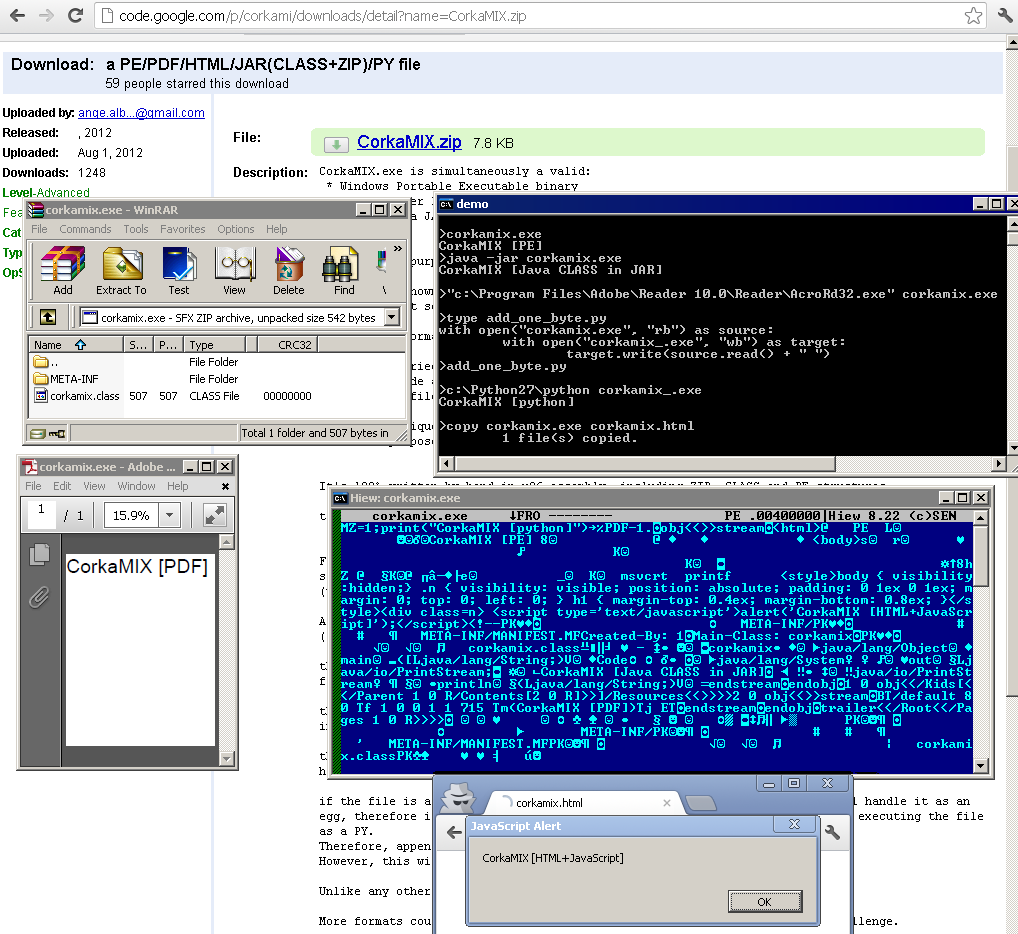
\includegraphics[width=0.7\textwidth]{albertini/img/corkamix}
  \caption{Un joli \emph{patchwork}}
  \label{fig:albertini:corkamix}
\end{figure}

On peut rajouter de nombreux formats dans le fichier \ZIP lui-même, mais ça ne présente aucun challenge particulier.

Un tel mélange binaire ne nécessite pas de faire ces fichiers à la main: on peut prendre des fichiers tout à fait standards et obtenir un résultat analogue, bien qu'ayant un air plus familier (figure~\ref{fig:albertini:sssticmix}).

\begin{figure}[p]
  \centering
  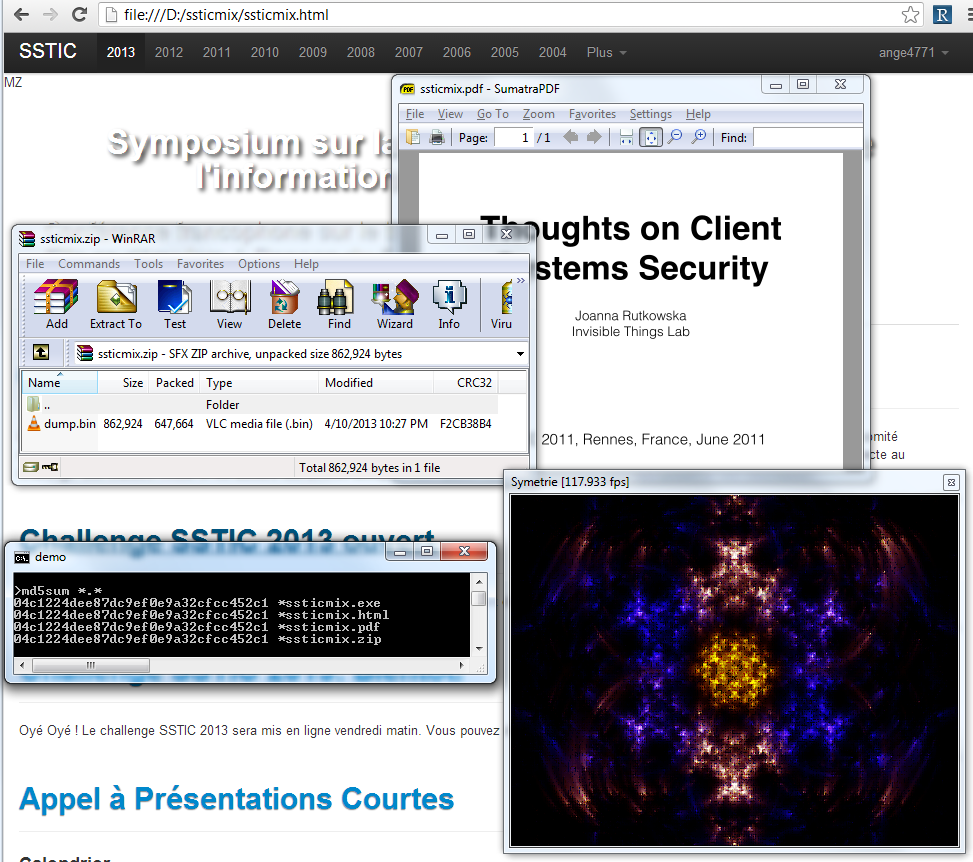
\includegraphics[width=0.7\textwidth]{albertini/img/sssticmix}
  \caption{Un polyglotte binaire avec un air familier.}
  \label{fig:albertini:sssticmix}
\end{figure}

\subsection{Autres systèmes d'exploitations}

Un esprit moqueur serait tenté de se contenter de blâmer \emph{Microsoft} et \emph{Adobe} pour leur laxisme, et le fait d'accepter ainsi n'importe quel format binaire.

\subsubsection{Linux}

En regardant le format \PDF dans un premier temps, on s'aperçoit que les visionneuses \PDF standards sous Linux, bien que n'acceptant pas le \PDF particulier généré précedemment, n'en sont pas pour autant vraiment rigoureuses.

En effet, en creusant un peu, on s'aperçoit que de nombreux outils \PDF tels qu'Evince ou la visionneuse standard d'Ubuntu, acceptent un \PDF ne contenant même pas de signature \texttt{\%PDF} --- même partielle --- ce qu'\emph{Adobe Reader} refusera immédiatement.

Le format binaire Linux, {\it Executable File Format} --- dit \ELF --- n'impose rien de particulier concernant le fichier lui-même. Créer un tel polyglotte basé sur un \ELF plutôt qu'un \PE ne présente alors pas de difficulté particulière, tel que le montre la figure \ref{fig:albertini:corkaminux}.

\begin{figure}[p]
  \centering
  \includegraphics[width=0.7\textwidth]{albertini/img/corkaminux}
  \caption{Un polyglotte binaire sous Linux.}
  \label{fig:albertini:corkaminux}
\end{figure}


\subsubsection{Mac OS X}

Les visionneuses \PDF standards Mac OS X et iOS sont elles, beaucoup plus strictes.

Elles refusent toute signature incomplète ou absente. Les seules malformations théoriques acceptées sont l'absence de \texttt{xref}, longueurs de flux (\texttt{stream /length}), et signature de fin de fichier \texttt{\%\%EOF}.

Le format binaire de Mac OS X, le \MACHO (pour \emph{Mach Object}) ne présente, à l'instar des formats \PE et \ELF, aucune difficulté particulière une fois qu'on a la maîtrise de leur structure binaire (figure~\ref{fig:albertini:corkamosx}).
\begin{figure}[p]
  \centering
  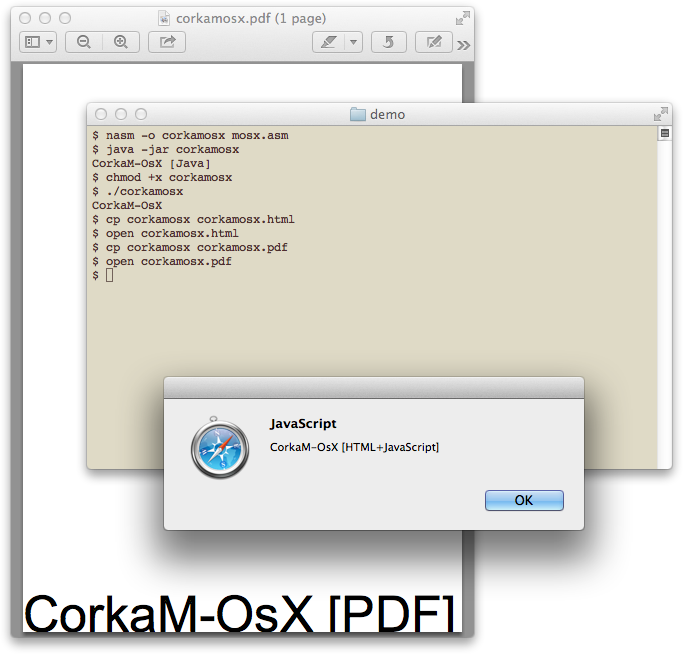
\includegraphics[width=0.7\textwidth]{albertini/img/corkamosx}
  \caption{Un polyglotte binaire sous Mac OS X.}
  \label{fig:albertini:corkamosx}
\end{figure}


\subsection{comparaison d'autres visionneuses \PDF répandues}

Bien que le standard \PDF soit publiquement défini, chaque visionneuse tolère des malformations particulières.

Ceci peut être exploité pour créer un document qui contient un code malveillant qui ne sera vu et traité que par une visionneuse spécifique.

En examinant des visionneuses standards telles que {\em Sumatra}, {\em Chrome} et {\em Adobe Reader}, on s'aperçoit qu'il est possible de faire un document, qui, bien que fonctionnant sans problème sous les trois, se révèle en fait être composé de trois documents indépendants fusionnés, dont chaque élément co-existe en s'ignorant (cf figures~\ref{fig:albertini:pdf-pdf_standardmerged}~et~\ref{fig:albertini:pdf-standard}).

\begin{figure}[ht]
  \centering
  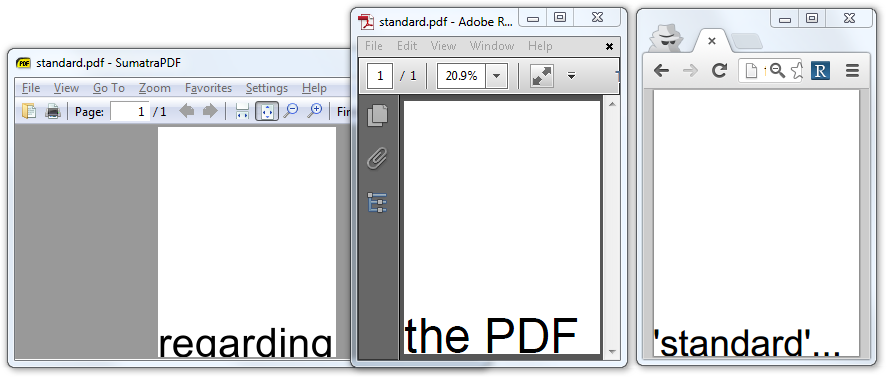
\includegraphics[width=0.8\textwidth]{albertini/img/pdf_standardmerged}
  \caption{Un document interprété différemment par 3 visionneuses distinctes.}
  \label{fig:albertini:pdf-pdf_standardmerged}
\end{figure}

Chaque élément spécifique à une visionneuse étant ignoré par les autres, on peut donc le mutiler au maximum, ce qui fait qu'il pourrait être perçu comme corrompu, et ainsi passer outre des filtres de sécurité: la figure~\ref{fig:albertini:pdf-standard} met en valeur les différences de chaque élement, et ainsi les largesses de chaque visionneuse par rapport aux autres.

\begin{figure}[ht]
  \centering
  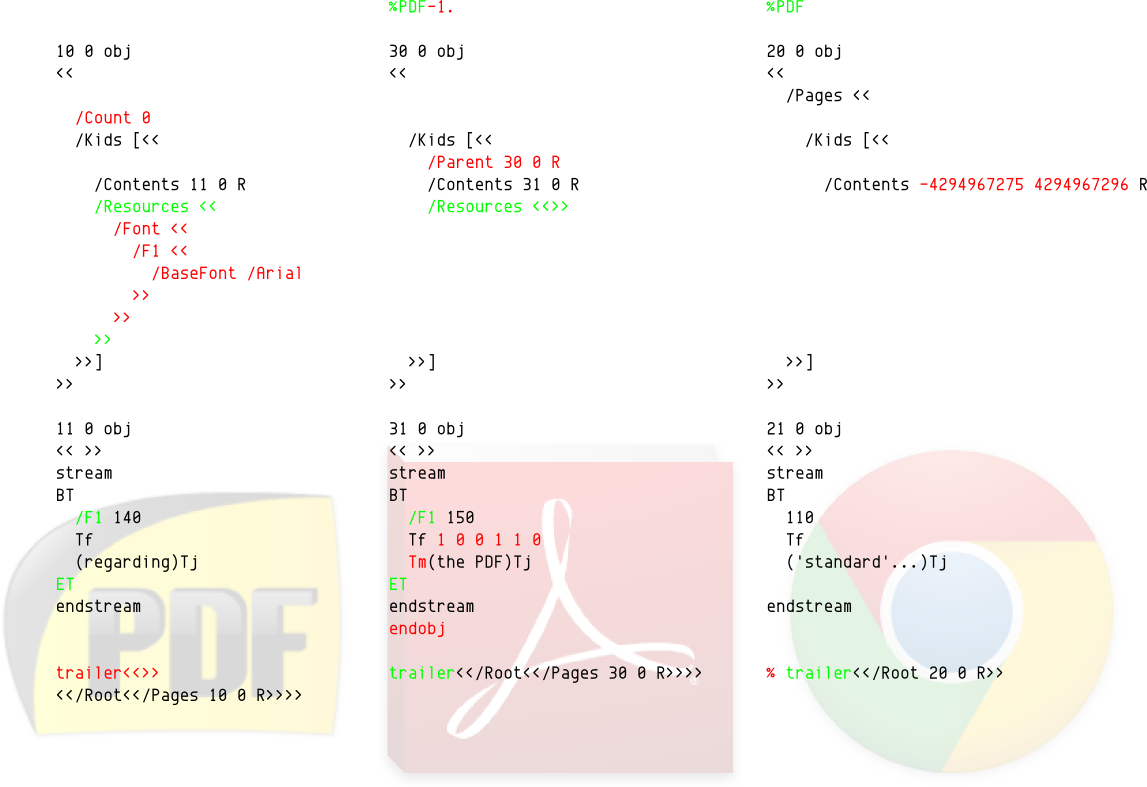
\includegraphics[width=0.8\textwidth]{albertini/img/pdf-standard}
  \caption{Comparaison des différences possibles entre 3 visionneuses.}
  \label{fig:albertini:pdf-standard}
\end{figure}

La visionneuse {\em PDF.JS} est un cas à part: elle bien plus stricte que toutes les autres. Notamment, elle impose~:

\begin{itemize}
\item une table de références \texttt{xref}.
\item une longueur déclarée à chaque \texttt{stream}.
\end{itemize}

qui sont des éléments dont l'absence est tolérée par toutes les autres.

\section{Conséquences pour la sécurité}
Tels des marques de lessive, les outils de sécurité sont comparés selon de trop simples critères: vitesse d'analyse et taux de détection d'un même ensemble empirique de fichiers.

Tout outil d'analyse commercial grand public a donc la lourde responsabilité de ne pas trop s'attarder sur un fichier particulier. En conséquence, il est crucial que le moteur de celui-ci détecte au plus tôt, et efficacement, le type du fichier analysé.

On peut donc imaginer le début de l'exécution d'un tel outil comme une grosse gare de triage: il n'est donc pas surprenant qu'un fichier, une fois détecté comme correspondant à un format connu (comme le montre la figure \ref{fig:albertini:corkamix-vt}), sera analysé comme tel, et donc ne sera pas réanalysé par la suite comme étant d'un autre format.

\begin{figure}[ht]
  \centering
  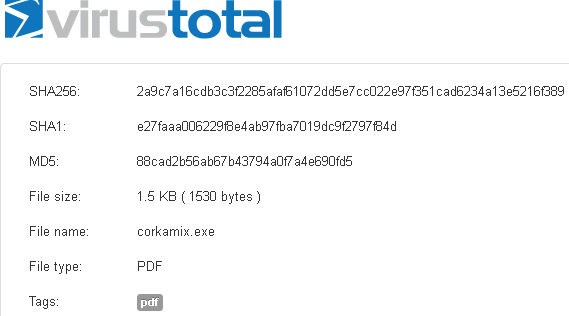
\includegraphics[width=0.8\textwidth]{albertini/img/corkamix-vt}
  \caption{Un exécutable identifié uniquement comme \PDF.}
  \label{fig:albertini:corkamix-vt}
\end{figure}

Quand bien même il le serait, l'outil ne va pouvoir se permettre de réanalyser totalement le fichier comme étant d'un autre format, car il va au bout d'un moment couper l'analyse, pour ne pas s'attarder trop longtemps sur un seul fichier.

Soit la machine qui traite le fichier passe beaucoup de temps (déni de service sur l'anti-virus, ou du moins perte de qualité en matière de vitesse aux yeux des magazines informatiques, ce qui est hors de question pour un produit commercial),
soit l'anti-virus jette un fichier qu'il ne peut analyser de manière exhaustive (déni de service sur la passerelle de fichiers, qui est généralement jugé inacceptable).

Une première démarche pour l'auteur de virus est donc de légitimement feindre un format de fichier: l'outil de sécurité analysera ce fichier comme tel, puis, ne trouvant rien de malveillant dans ce format particulier, déclarera le fichier comme sain.
Ça peut donc se faire simplement en commençant un fichier par la signature \PE,
puis en continuant le fichier comme un fichier \HTML ou \PDF.

De plus, certains outils utilisent un système de cache pour savoir s'ils ont déjà analysé un fichier. Donc, la réutilisation du même fichier --- même sous un autre format --- sautera toute nouvelle analyse via une interception dynamique lors de l'exécution.

Puisqu'un outil de sécurité se doit d'être le plus rapide possible et le plus simple possible, il ne rend comme verdict qu'un booléen, sans tenir compte du format possible du fichier: un booléen par fichier, et non par type possible de fichier.
Le vrai problème, c'est qu'un autre logiciel vulnérable, tel que \JAVA, une visionneuse \PDF ou un navigateur, va peut-être interpréter ce fichier de manière différente.


Une deuxième démarche consiste à inclure un maximum de format, pour que, quelque soit l'ordre d'analyse de l'outil, il atteigne sa limite imposée de temps/cycles, et ainsi qu'il abandonne avant d'avoir pu déterminer si le fichier est sain ou non.

Une autre possibilité est que le fichier cause des problèmes au moteur de l'outil, et qu'il échoue directement.

La première priorité pour un outil de sécurité est de déterminer au plus tôt qu'il y a une combinaison inhabituelle de formats binaires dans un seul fichier, ce qui augmente la suspicion. Si cette combinaison ne concerne aucun cas légitime, tels qu'un \HTML combiné à un exécutable \PE, le fichier peut être classé comme malveillant selon cet unique critère. Malheureusement, cette combinaison de formats peut être perçue comme un avantage technique par des développeurs peu renseignés, et, bien que déconseillée en pratique, peut être rencontrée dans la nature.

D'autre part, tous les navigateurs modernes analysent l'intégralité d'un fichier pour son contenu Web, même s'il est hors norme: par exemple, un fichier constitué d'un exécutable \PE de 27~Mo suivi d'une page Web fonctionnera toujours dans les 2 formats. Un outil de sécurité grand public se devra de se limiter {\it a priori} aux premiers méga-octets, pour optimiser sa performance.

\begin{figure}[ht]
  \centering
  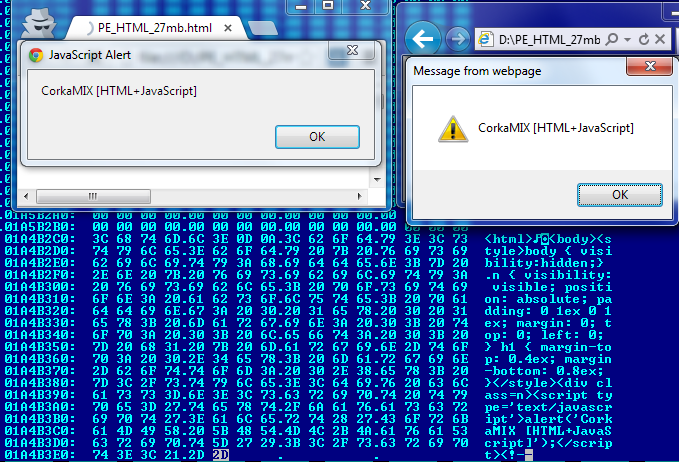
\includegraphics[width=0.8\textwidth]{albertini/img/PE_HTML_27mb}
  \caption{Une page \HTML à la suite d'un \PE de 27Mo.}
  \label{fig:albertini:PE_HTML_27mb}
\end{figure}


\section{Conclusion}

Bien que la plupart excluent d'être combinés à d'autres, certains formats de fichiers autorisent des largesses, ce qui rend la combinaison de formats binaires dans un seul fichier possible.

Ceci a des conséquences de sécurité importantes liées à la confusion entre formats: exécution de virus via les navigateurs, exfiltration de fichier, abandon de l'analyse par les outils de sécurité, menant à considérer un fichier malveillant comme sain (de plus, les malformations possibles de ces formats compliquent l'analyse automatisée et manuelle de virus).

Il semble donc indispensable de ne créer que des standards déterminés par une signature unique au début du fichier.

\emph{Adobe Reader} rejette d'ailleurs, depuis la version 10.1.5 de janvier 2013, tout fichier \PDF commençant par une signature connue telle que \PE, \emph{PNG}, \emph{JPG} \ldots Il ne devrait pourtant en théorie n'accepter que les \PDF commençant par une signature \PDF, mais ce n'est souvent pas le cas dans la pratique.

Les autres visionneuses (\emph{Chrome}, \emph{Sumatra}, \emph{Evince}) acceptent toujours n'importe quel début de fichier. En particulier, \emph{Sumatra} est devenu récemment (version 2.2) plus laxiste en tolérant l'absence de \texttt{endobj} après \texttt{endstream}, alors qu'\emph{Adobe Reader}, au contraire, et comme on s'y attend, renforce progressivement les contrôles de la structure du document.

Une autre possibilité serait d'imposer au système le type de fichier: quand un fichier est téléchargé, il est étiqueté comme son type original, et ensuite le système impose son type, tant qu'une opération externe de dévérouillage de type n'a pas été effectuée.

De même, l'exécution d'un fichier via les APIs \WIN n'impose aucune extension, ce qui rend les exécutables --- pourtant omniprésents dans les virus --- plus facile à lancer, alors qu'il n'y a pas de raison fondamentale qu'on accepte de lancer comme un \PE un document \PDF ou une page \HTML.

\bibliography{albertini/biblio}

%%% Local Variables:
%%% mode: TeX-PDF
%%% TeX-master: "master"
%%% End:


%\tableofcontents
\mainmatter


\settitle[CorkaMIX]{Polyglottes binaires et implications}

\newcommand{\TODO}[1]{}
%\newcommand{\TODO}[1]{\textcolor{red}{TODO:~#1}}

\newcommand{\WIN}[0]{\emph{Windows}\xspace}

\newcommand{\ZIP}[0]{\emph{ZIP}\xspace}
\newcommand{\JAVA}[0]{\emph{Java}\xspace}
\newcommand{\GIF}[0]{\emph{GIF}\xspace}
\newcommand{\PE}[0]{\emph{PE}\xspace}
\newcommand{\ELF}[0]{\emph{ELF}\xspace}
\newcommand{\MACHO}[0]{\emph{Mach-O}\xspace}
\newcommand{\JAR}[0]{\emph{JAR}\xspace}
\newcommand{\HTML}[0]{\emph{HTML}\xspace}
\newcommand{\PDF}[0]{\emph{PDF}\xspace}

\setauthor[Ange~Albertini]{Ange Albertini\\
  \email{ange.albertini@gmail.com}}
\institute{Corkami.com}


\maketitle

\begin{abstract}
De l'exploitation à l'infection, les {\it malwares} modernes utilisent de nombreux formats de fichier binaires.
Il est crucial de pouvoir correctement les identifier et les analyser, si possible de manière automatique.
Bien que ces formats soient a priori clairement différenciés, il est parfois possible de combiner certains d'entre eux dans un seul et même fichier.
On parle alors de fichiers {\it polyglottes}.
De tels fichiers {\it polyglottes} ont donc dans un premier temps été créés.
Ensuite, plusieurs caractéristiques non documentées de chaque format concerné ont été rajoutées, pour mettre en évidence l'importance du problème entre les limites des documentations officielles, et la réalité (du monde des virus).
Les conséquences sur le fonctionnement des outils de sécurité sont finalement mises en évidence, avec ce que ça implique pour l'utilisateur final.
\end{abstract}


\section{Introduction}

\subsection{État de l'art}

Un fichier polyglotte est un fichier qui peut être interprété dans plusieurs langages différents.  Un des plus simple d'entre eux, représenté par le Polyglot de David Kendall dans le listing~\ref{lst:albertini:polyglot}, fonctionne en Ruby, Perl, PHP, ksh, Scheme, Lisp, Clojure, Plan. Les {\it polyglottes} peuvent aller beaucoup plus loin, jouant sur les différences d'interprétation et de {\it pré-processing} de chaque langage inclus dans le fichier.


\begin{lstlisting}[language={},caption={Un programme polyglotte simple.},label={lst:albertini:polyglot}]
 (print "Hello, world!\n");
\end{lstlisting}

La première utilisation de fichiers polyglottes dans le monde des virus est GIFAR~\cite{albertini:wikipedia:gifar}~:

un GIFAR résulte de l'ajout d'une classe \JAVA stockée au format \JAR à la suite d'une image au format \GIF. En effet, le \GIF est un format d'image couramment utilisé sur le Web, notamment pour les avatars dans les forums de discussion. Une fois le fichier sur le serveur, il est ensuite utilisable aussi comme une classe \JAVA. Si on utilise cette classe dans un script quelconque sur le serveur, le navigateur laissera accèder à la classe, même si elle est malveillante, car elle est maintenant hébergée sur le même site.

Julia Wolf~\cite{albertini:wolf:omgwtfpdf} a introduit le concept de \ZIP et \emph{Portable Document Format} --- dit \PDF --- combinés, ce qui permet de tromper les outils de sécurité et ainsi permettre d'exfiltrer des informations, ou passer pour un fichier innocent.

Jonas Magazinius~\cite{albertini:magazinius:polyglots} s'est également penché sur la question, en combinant notamment image \emph{JPG} et document \PDF.

En revanche, les formats de fichiers binaires sont, eux, rarement compatibles, car exclusifs: en effet, la majeure partie d'entre eux doivent nécessairement débuter par un marqueur (on parle aussi de \emph{magic number} en anglais), spécifique à chaque format, à de rares exceptions près (tel {\tt 0xcafebabe}, pour le format \MACHO universel et les classes \JAVA).

Il ne semble donc pas possible de combiner des formats binaires en général. Cependant, il y a quelques exceptions:
\begin {itemize}
\item tout d'abord, certains formats de fichier n'ont aucun en-tête, tels que le \emph{Master Boot Record} --- dit \emph{MBR} --- ou les fichiers \emph{COMMAND FILE} --- dit \emph{COM}. Il est donc possible de créer un secteur de démarrage à la fois au format \emph{GRUB} et au format \emph{MBR}~\cite{albertini:scott:metalkiller}, ou bien un fichier \emph{COM} qui soit également un fichier exécutable linux \ELF.

\item d'autre parts, d'autre formats de fichiers n'imposent pas que le marqueur soit présent au début du fichier: c'est le cas des archives (\ZIP, \emph{RAR}\ldots), des pages \HTML, et des documents \PDF.

\item enfin, certains formats, bien que commencant obligatoirement au premier déplacement, autorisent un grand espace entièrement modifiable juste après la signature, tels que le format d'exécutable \emph{Portable Executable} --- dit \PE --- et le format d'image \emph{PICT}.
\end{itemize}

Hélas, certains formats utilisables à des fins malveillantes sont librement combinables dans un seul et même fichier, mais de plus, il s'agit des formats parmi les plus utilisés ces dernières années pour la prolifération de {\it malware}:
en effet, la chaîne d'infection complète par un virus la plus répandue est une page \HTML, contenant du Javascript, qui va charger un fichier \JAVA profitant d'une vulnérabilité, qui lui-même va télécharger le virus final, sous forme d'un exécutable \WIN, au format \emph{PE} --- et on peut effectivement combiner une page \HTML, une classe \JAVA, et un fichier binaire au format \PE.

Un autre vecteur d'infection répandu est un \PDF activant une vulnérabilité, dont le \emph{shellcode} téléchargera un \PE. Et là encore, \PE et \PDF sont combinables dans un seul et même fichier.

\subsection{Pivot}

Le format pivot de la grande majeure partie des virus est le format de binaire universel de \WIN, le format \PE. Pour ce rôle unique dans la chaîne virale, il a donc été choisi comme point de départ.

\section{Exploration du format \PE}
Ce format stipule que le fichier commence par une structure \texttt{IMAGE\_DOS\_HEADER}, de \texttt{0x40} octets:
\begin{itemize}
\item les 2 premiers octets de cette structure définissent un champ appelé \texttt{e\_magic}, qui contient obligatoirement la signature \texttt{MZ}~: Il est donc impossible de le combiner à tout autre format imposant une signature spécifique au déplacement 0.
\item tous les champs suivants, à l'exception du dernier, ne concernent que la fonctionnalité \emph{DOS} de l'exécutable --- qui se borne en majeure partie à afficher un message d'erreur. Elle est totalement ignorée quand le fichier est chargé en tant que \PE.
\item le dernier champ, \texttt{e\_lfanew}, est un pointeur sur 32 bits vers la structure suivante de l'exécutable.
\end{itemize}

On sait donc que notre fichier doit commencer par {\tt M} et {\tt Z}, et qu'au déplacement \texttt{0x3C} doit se trouver un pointeur. Entre les deux, on peut y faire ce que l'on veut, tout en gardant la fonctionalité \PE intacte. On peut même mettre l'en-tête \PE à la fin du fichier sans problème.

\subsection{Création d'une page \HTML dans un exécutable}

Le laxisme omniprésent dans les pages \HTML fait qu'au final, les navigateurs se contentent d'ignorer un peu tout --- quand bien même ce serait de l'information non encodable en \emph{ASCII} --- au cas où un tag \texttt{<HTML>} finirait par être présent.

Ainsi, le simple fait de rajouter à la fin d'un exécutable du code \HTML va en faire une page web fonctionnelle, pour peu qu'on renomme l'extension du fichier, comme le montre la figure~\ref{fig:albertini:htmlnotepad}.

\begin{figure}[ht]
  \centering
  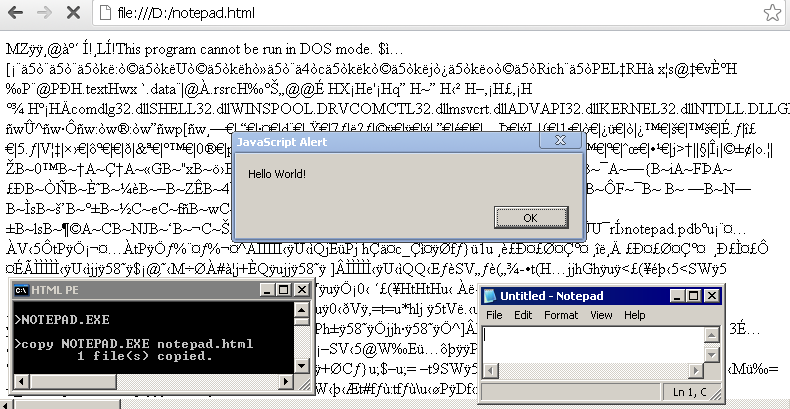
\includegraphics[width=0.8\textwidth]{albertini/img/htmlnotepad}
  \caption{Le bloc-note \WIN avec une page HTML ajoutée à la fin.}
  \label{fig:albertini:htmlnotepad}
\end{figure}

Cela dit, bien que le fichier soit fonctionnel dans les deux formats, les données binaires perturbent l'affichage de la page web, bien que celles-ci soient placées avant le tag ouvrant \texttt{<HTML>}.
On va donc jouer sur les \emph{Cascaded Style Sheet} pour effacer ces données et ainsi avoir un résultat visuellement parfait. Ou sinon, on peut insérer ce tag juste après la signature du \PE, auquel cas on aura juste un \texttt{MZ} affiché sur la page.

De même, si on souhaite rajouter quelque chose après la page web et son script, il nous suffit d'ouvrir un bloc de commentaire non fermé \texttt{<!----}.

À noter que si une page web doit avoir une extension précise pour être visualisée correctement, un exécutable \WIN n'a besoin d'aucune extension particulière pour être exécuté via les APIs \WIN.

\subsection{Concaténation d'un \PDF et d'un exécutable}

La spécification officielle stipule que la première ligne d'un \PDF doit être sa signature:
\begin{center}
  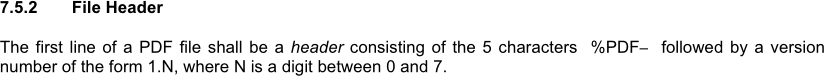
\includegraphics[width=0.8\textwidth]{albertini/img/pdfsigtheory}
\end{center}

En pratique, il n'en n'est rien, il est juste requis sous \emph{Adobe Reader} qu'une signature valide soit présente dans les 1024 (\texttt{0x400}) premiers octets.

\begin{figure}[ht]
  \centering
  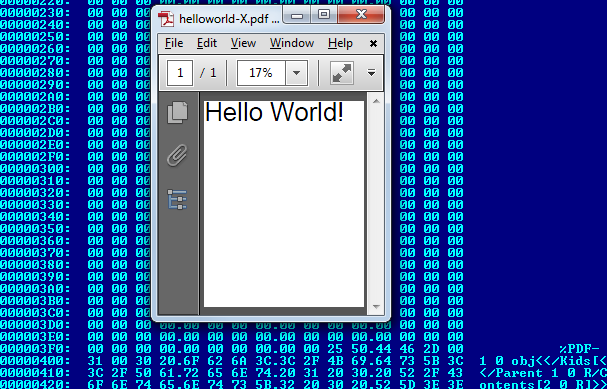
\includegraphics[width=0.8\textwidth]{albertini/img/pdfsigpractice}
  \caption{Un \PDF dont la signature est à la fin des \texttt{1024} premiers octets est toujours reconnu par \emph{Adobe Reader}.}
  \label{fig:albertini:pdfsigpractice}
\end{figure}

On peut donc, dans un premier temps, rajouter à la fin d'un petit exécutable un \PDF dans son intégralité, et les deux fonctionneront encore comme on s'y attend, comme dans la figure~\ref{fig:albertini:tinyPEPDF}.

\begin{figure}[ht]
  \centering
  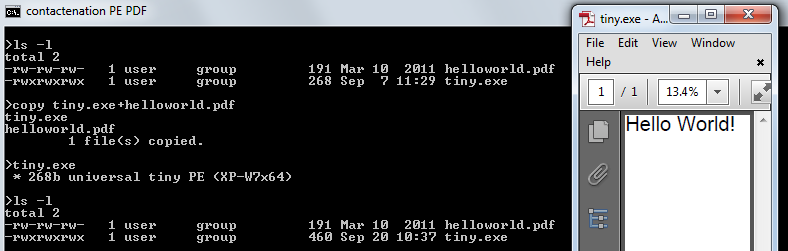
\includegraphics[width=0.8\textwidth]{albertini/img/tinyPEPDF}
  \caption{Un \PDF greffé à la fin d'un petit exécutable \PE.}
  \label{fig:albertini:tinyPEPDF}
\end{figure}

Dans le cas d'un \PE plus gros que \texttt{1024} octets, on devra rajouter la signature \PDF dans l'en-tête \PE.

Il arrive cependant que le \PE, stocké au format binaire, contienne des séquences de caractères qui seront interprétées par la visionneuse \PDF. Pour cela, il suffit d'entourer le reste du \PE d'une structure d'objet \emph{stream} fictive, et ainsi son contenu ne sera pas analysé, puisqu'il n'est pas référencé dans la hiérarchie du document, comme dans la figure~\ref{fig:albertini:pdfnotepad}.

\begin{figure}[ht]
  \centering
  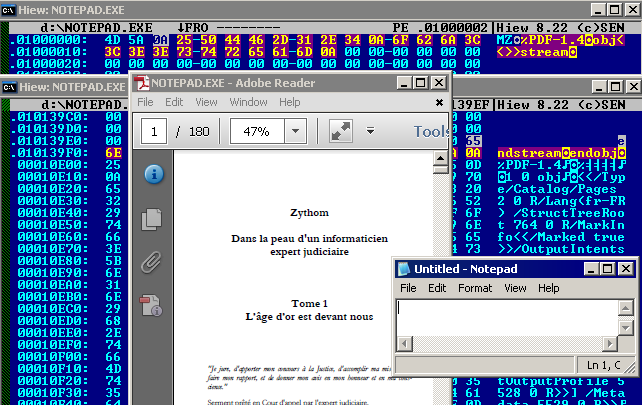
\includegraphics[width=0.8\textwidth]{albertini/img/pdfnotepad}
  \caption{Le bloc-note \WIN avec un fichier \PDF ajouté à la fin.}
  \label{fig:albertini:pdfnotepad}
\end{figure}


\subsection{Une archive \ZIP dans un exécutable}
Le format \ZIP n'impose rien quant au début du fichier --- il est lu en partant de la fin, et tolère des données avant ou après la structure du format elle-même. Un fichier \ZIP peut donc se trouver n'importe où dans un autre fichier.

Une classe \JAVA peut être exécutée directement, ou en étant contenue dans un fichier {\em Java Archive}, dit \JAR.
Un fichier \JAR n'est qu'une archive \ZIP contenant une ou plusieurs classes \JAVA, et un fichier texte (\texttt{manifest}) au contenu bien défini.

Contrairement à un \ZIP standard, un fichier \JAR doit terminer strictement le fichier: si on rajoute ne serait-ce qu'un seul octet à la suite, \JAVA ne reconnaît plus ce fichier comme valide.

\subsection{Récapitulons}

À l'aide des manipulations décrites précédemment, nous obtenons donc:
\begin{enumerate}
\item le début d'un \PE
\item une signature \PDF dans ses \texttt{1024 - 6} premier octets
\item la suite du \PE, inclue dans un objet \texttt{stream} \PDF
\item dans un ordre quelconque~:
\begin{itemize}
\item le reste du \PDF, finissant l'objet fictif
\item la page \HTML
\end{itemize}
\item un \ZIP, optionnellement un \JAR
\end{enumerate}

\section{Détails de mise en oeuvre}

Un simple fichier polyglotte est donc faisable via des opérations de concaténations et quelques modifications manuelles.

Pour pousser l'expérience quant au comportements d'outils de sécurité, des propriétés anormales seront ajoutées aux formats inclus, dans le but de tester leur robustesse.

Afin d'y arriver, l'intégralité du fichier sera faite à la main, pour en garder le contrôle complet.

Toutes les structures sont crées à partir de zéro, en assembleur: en effet, un assembleur standard a la possibilité de définir chaque octet manuellement, et aussi de créer des fonctions et des structures, qui vont faciliter la création du fichier, tout en gardant le contrôle de chaque octet.

Quand un fichier est stocké dans une archive \ZIP sans compression, il est stocké dans son intégralité, à l'identique: inclure un fichier dans une archive ne revient donc qu'à ajouter en-tête et pied de page.

\subsection{Un \PE fait main}

\subsubsection*{Peu d'éléments définis}

Notre exécutable contient \texttt{Hello World} compilé en assembleur standard, mais seulement 18 éléments sont absolument indispensables, toutes structures confondues, tel que le montre la figure~\ref{fig:albertini:empty_pe_header}.

\begin{figure}[ht]
  \centering
  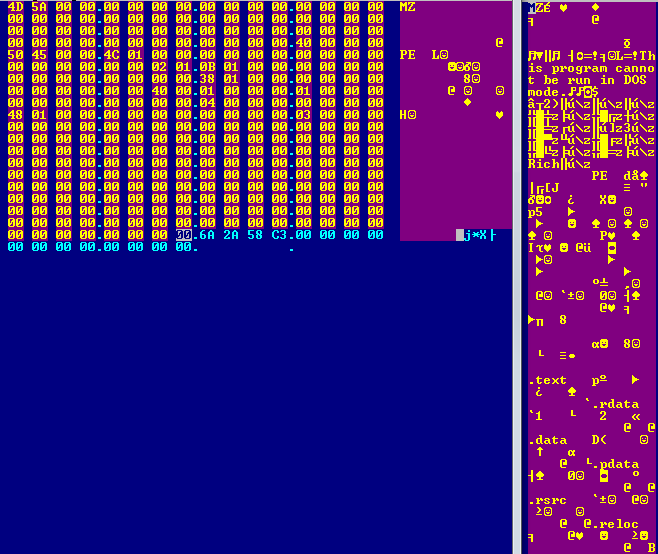
\includegraphics[width=0.8\textwidth]{albertini/img/empty_pe_header}
  \caption{Comparaison d'en-têtes \PE.}
  \label{fig:albertini:empty_pe_header}
\end{figure}

On obtient donc un \PE qui va faire échouer les outils naïfs qui déterminent la validité du fichier d'après des éléments non indispensables.

\subsubsection*{Pas de sections}

Quand un exécutable utilise des alignements faibles, tout l'exécutable est chargé en mémoire indépendamment de la table des sections. Il devient dans ce cas possible de ne définir aucune section (\emph{NumberOfSections = 0}), et de ne pas avoir de table de section (\emph{SizeOfOptionalHeader = 0}).

Là encore, il fera échouer les outils qui analysent ce format section par section.

\subsubsection*{Utilisation d'instructions non documentées}

Un outil de sécurité avancé va essayer d'émuler l'exécution du début du fichier, pour déterminer s'il est malveillant ou non.

Certaines instructions, non documentées, peuvent amener un tel émulateur à abandonner, car il ne peut déterminer comment procéder. La présence de telles instructions ne peut vraisemblablement pas amener à qualifier le fichier de malveillant, car il pourrait s'agir de nouvelles instructions d'un processeur récent.

Certaines de ces instructions comme {\tt SetALC} ou les {\tt nop} multi-octets sont absentes de la documentation Intel (figures~\ref{fig:albertini:undoc_setalc} et \ref{fig:albertini:undoc_nop}), mais présentes dans la documentation AMD (figures~\ref{fig:albertini:salc_amd} et \ref{fig:albertini:nop_amd}), parfois uniquement sous le status \emph{réservé}.


Ces instructions ne sont reconnues dans aucun outil Microsoft (figure~\ref{fig:albertini:corkamix_windbg}), car ils suivent la documentation Intel à la lettre.


\begin{figure}[ht]
  \centering
  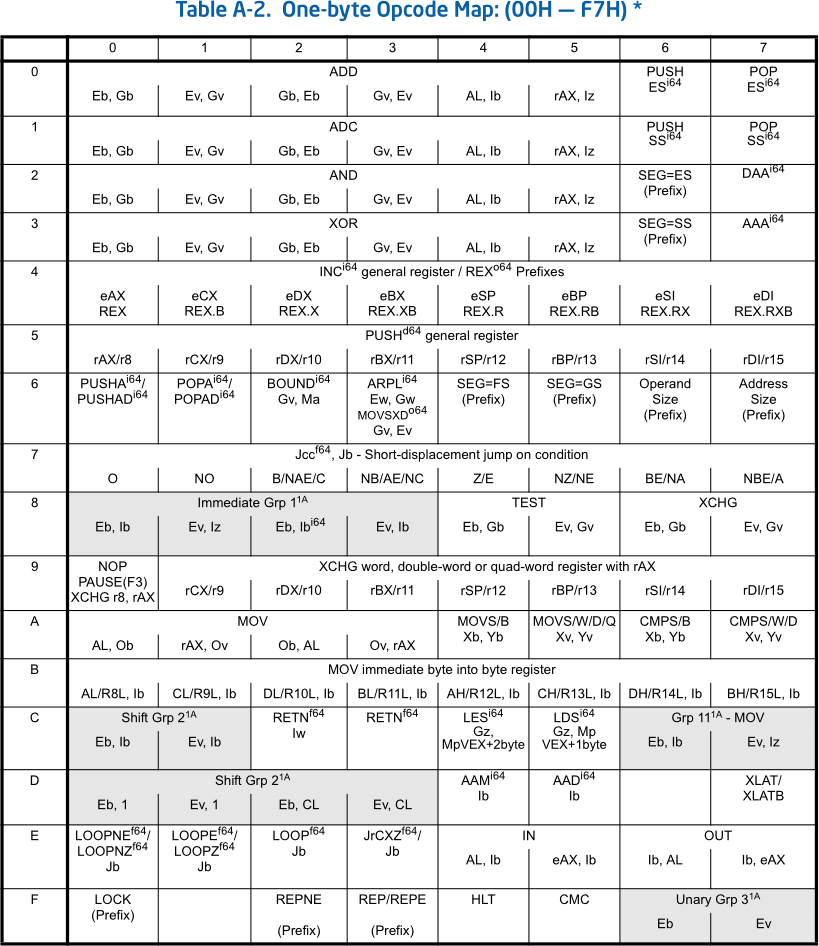
\includegraphics[width=0.8\textwidth]{albertini/img/undoc_setalc}
  \caption{La documentation officielle n'indique rien pour l'octet \texttt{D6}.}
  \label{fig:albertini:undoc_setalc}
\end{figure}

\begin{figure}[ht]
  \centering
  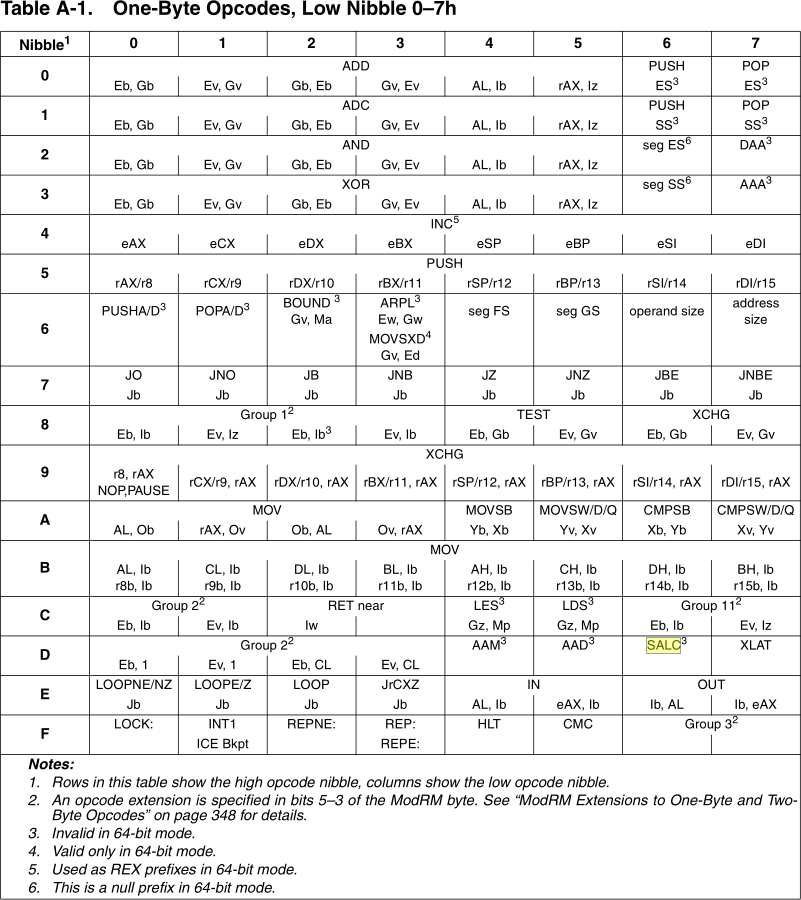
\includegraphics[width=0.8\textwidth]{albertini/img/salc_amd}
  \caption{SetALC est documenté par AMD.}
  \label{fig:albertini:salc_amd}
\end{figure}

\begin{figure}[ht]
  \centering
  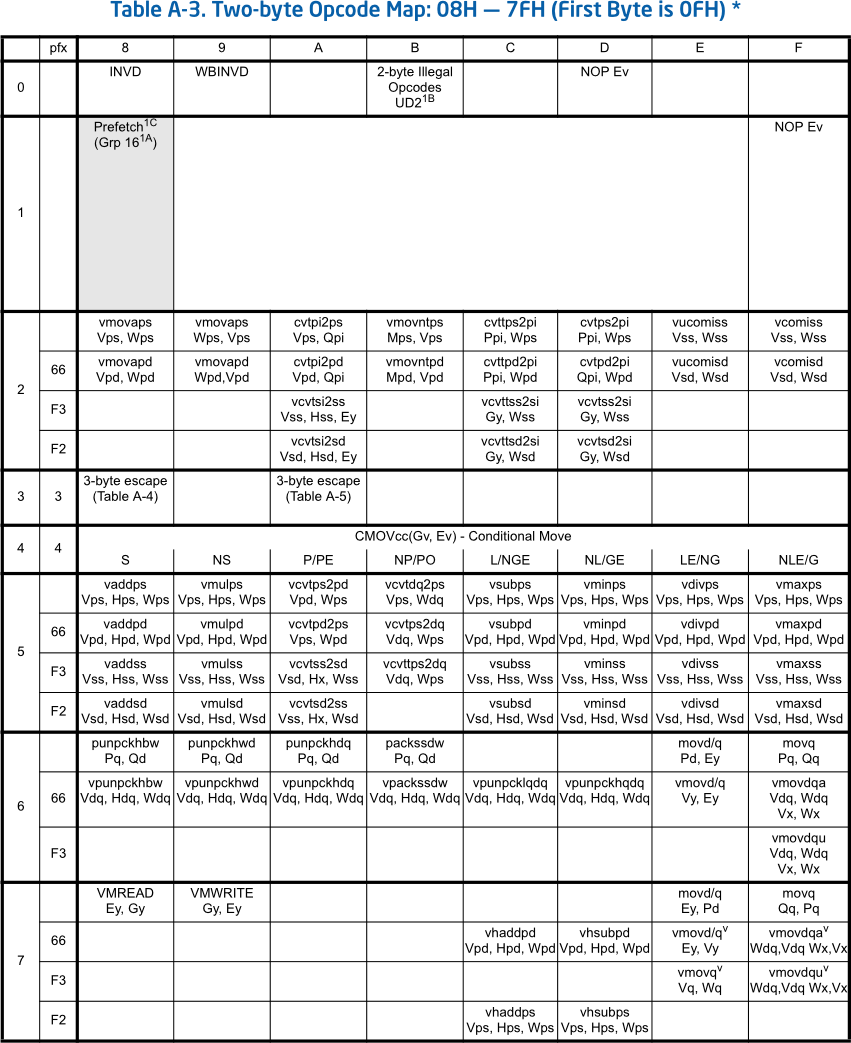
\includegraphics[width=0.8\textwidth]{albertini/img/undoc_nop}
  \caption{La documentation Intel ne mentionne NOP que pour les octets \texttt{0F 1F}.}
  \label{fig:albertini:undoc_nop}
\end{figure}

\begin{figure}[ht]
  \centering
  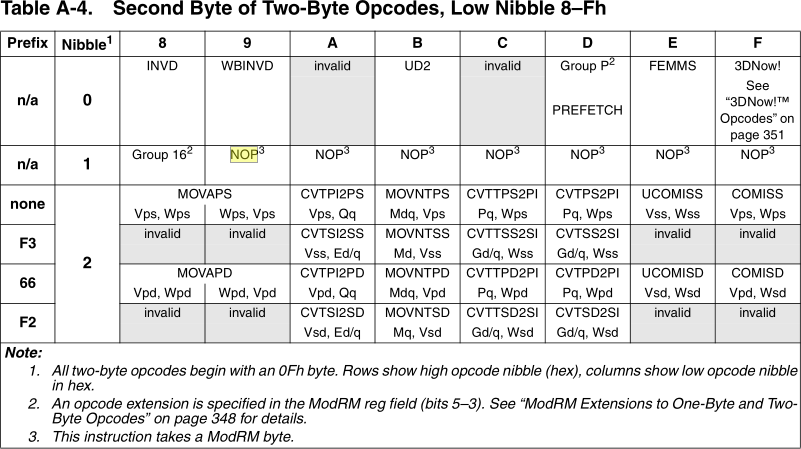
\includegraphics[width=0.8\textwidth]{albertini/img/nop_amd}
  \caption{Le NOP de plusieurs octets est complètement documenté par AMD.}
  \label{fig:albertini:nop_amd}
\end{figure}

\begin{figure}[p]
  \centering
  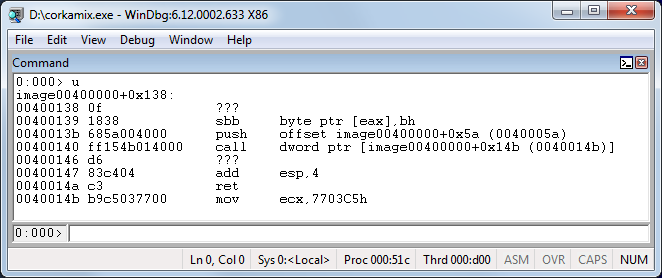
\includegraphics[width=0.8\textwidth]{albertini/img/corkamix_windbg}
  \caption{WinDbg montre plusieurs instructions inconnues.}
  \label{fig:albertini:corkamix_windbg}
\end{figure}

Pour implémenter ces instructions, on doit générer certaines à la main, un assembleur standard ne les gérant pas forcément.

\subsubsection*{Une structure d'import très compacte}

le \emph{DataDirectory} des imports pointe vers une liste de \emph{descripteurs}.
Cette liste se termine en théorie par un descripteur entièrement nul, mais en réalité uniquement si ses champs \texttt{Name} ou \texttt{FirstThunk} sont nuls.

La table des adresses, si elle est suffisamment petite, peut-être intégrée dans un des descripteurs, alors qu'elle utilise habituellement son propre espace du fichier.

De même, le nom de la DLL, même amputé de son extension, peut être inclus dans un des descripteurs, ainsi que la structure \texttt{IMAGE\_IMPORT\_BY\_NAME} de l'import, alors qu'eux aussi sont censés être instanciés séparément, hors des descripteurs.

On obtient donc une table d'import très compacte, avec beaucoup d'irrégularités, mais pourtant 100~\% gérée et fonctionnelle (figure~\ref{fig:albertini:imports}) par \WIN.

\begin{figure}[p]
  \centering
  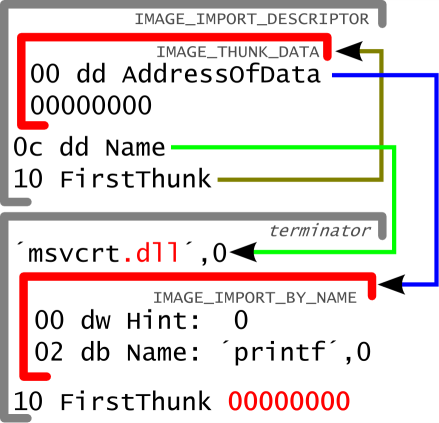
\includegraphics[width=0.5\textwidth]{albertini/img/imports}
  \caption{Une structure d'imports avec beaucoup de malformations.}
  \label{fig:albertini:imports}
\end{figure}

Ces astuces font que les outils les plus avancés échouent à analyser le \PE parfaitement. Notamment, à l'heure de création de ces recherches, la dernière version de Hiew et IDA échouent à les gérer (figure~\ref{fig:albertini:imports_error}).

\begin{figure}[p]
  \centering
  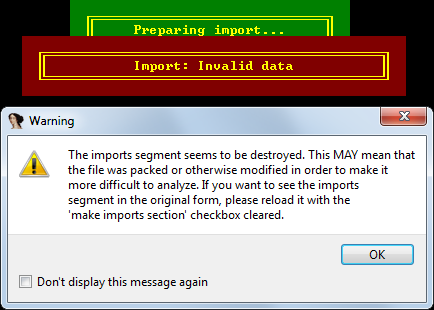
\includegraphics[width=0.5\textwidth]{albertini/img/imports_error}
  \caption{Une structure d'imports non gérée par Hiew ou IDA.}
  \label{fig:albertini:imports_error}
\end{figure}



\subsection{Un \PDF très compact}
La signature \PDF, bien qu'officiellement \texttt{\%PDF-1.?}, peut en fait être tronquée, selon la visionneuse employée.

La signature de fin \texttt{\%\%EOF} est absolument superflue, ansi que toute référence à une longueur dans les objets \texttt{stream}.

De même, la table \texttt{xref} est supprimable, ansi que les terminateurs d'objet \texttt{endobj}.

Enfin, le trailer final est réduit à son strict minimum.

On obtient donc, dans des cas extrêmes, un fichier \PDF particulièrement réduit de 36 octets fonctionnant sous Adobe Reader (listing~\ref{lst:albertini:tinypdf}).

\begin{lstlisting}[language={},caption={Un \PDF valide de 36 octets.},label={lst:albertini:tinypdf}]
%PDF- trailer<</Root<</Pages<<>>>>>>
\end{lstlisting}

\subsection{Un \emph{patchwork} binaire}

Au final, on obtient un fichier fonctionnel dans tous les formats inclus (figure~\ref{fig:albertini:corkamix}), et de nombreuses caractéristiques non documentées, qui font échouer des outils d'analyse et des anti-virus répandus.

\begin{figure}[p]
  \centering
  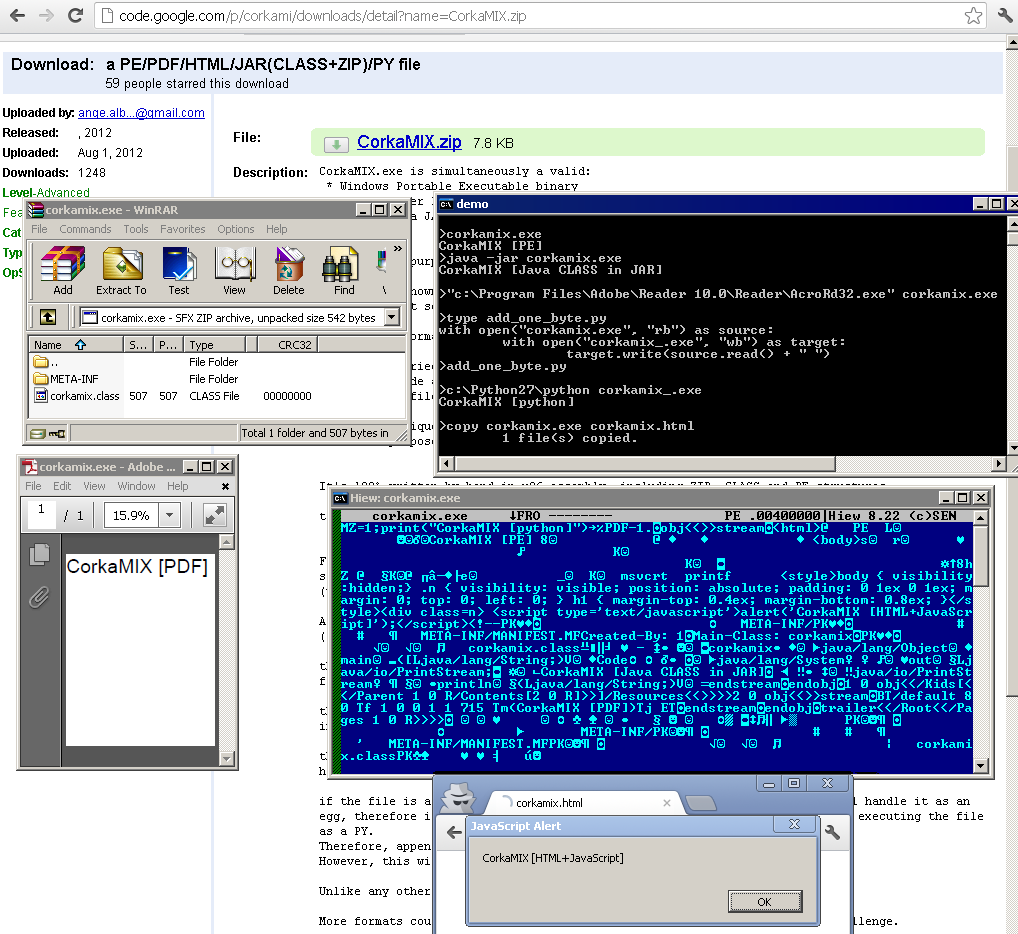
\includegraphics[width=0.7\textwidth]{albertini/img/corkamix}
  \caption{Un joli \emph{patchwork}}
  \label{fig:albertini:corkamix}
\end{figure}

On peut rajouter de nombreux formats dans le fichier \ZIP lui-même, mais ça ne présente aucun challenge particulier.

Un tel mélange binaire ne nécessite pas de faire ces fichiers à la main: on peut prendre des fichiers tout à fait standards et obtenir un résultat analogue, bien qu'ayant un air plus familier (figure~\ref{fig:albertini:sssticmix}).

\begin{figure}[p]
  \centering
  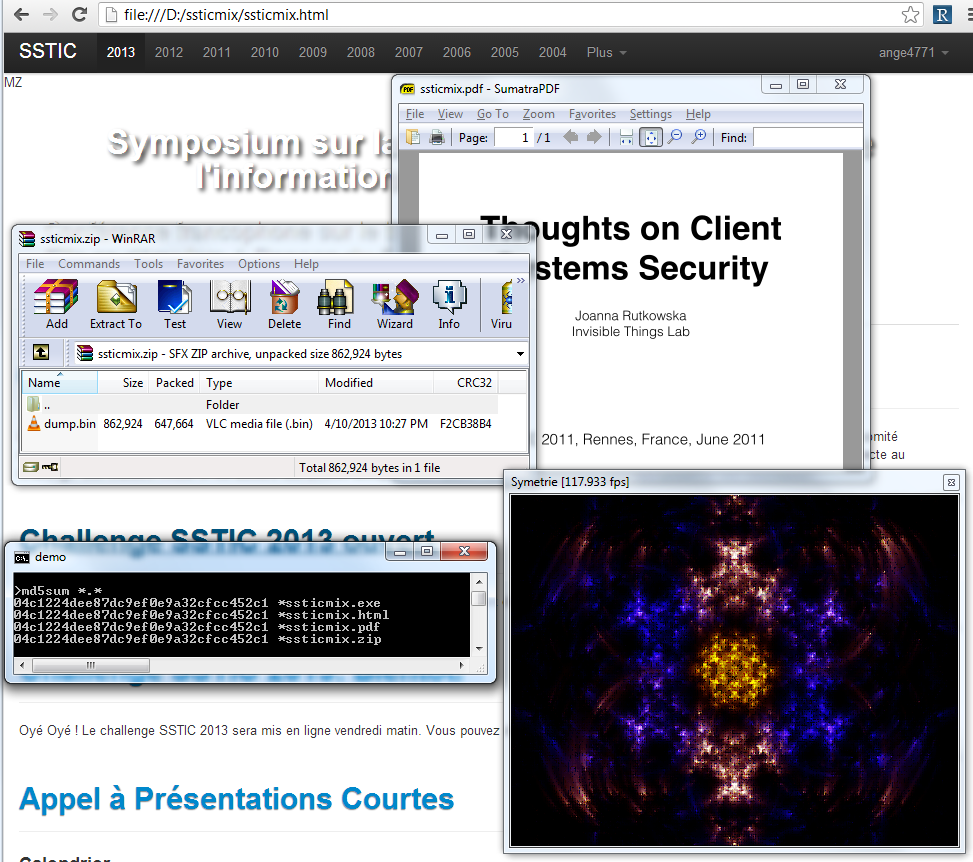
\includegraphics[width=0.7\textwidth]{albertini/img/sssticmix}
  \caption{Un polyglotte binaire avec un air familier.}
  \label{fig:albertini:sssticmix}
\end{figure}

\subsection{Autres systèmes d'exploitations}

Un esprit moqueur serait tenté de se contenter de blâmer \emph{Microsoft} et \emph{Adobe} pour leur laxisme, et le fait d'accepter ainsi n'importe quel format binaire.

\subsubsection{Linux}

En regardant le format \PDF dans un premier temps, on s'aperçoit que les visionneuses \PDF standards sous Linux, bien que n'acceptant pas le \PDF particulier généré précedemment, n'en sont pas pour autant vraiment rigoureuses.

En effet, en creusant un peu, on s'aperçoit que de nombreux outils \PDF tels qu'Evince ou la visionneuse standard d'Ubuntu, acceptent un \PDF ne contenant même pas de signature \texttt{\%PDF} --- même partielle --- ce qu'\emph{Adobe Reader} refusera immédiatement.

Le format binaire Linux, {\it Executable File Format} --- dit \ELF --- n'impose rien de particulier concernant le fichier lui-même. Créer un tel polyglotte basé sur un \ELF plutôt qu'un \PE ne présente alors pas de difficulté particulière, tel que le montre la figure \ref{fig:albertini:corkaminux}.

\begin{figure}[p]
  \centering
  \includegraphics[width=0.7\textwidth]{albertini/img/corkaminux}
  \caption{Un polyglotte binaire sous Linux.}
  \label{fig:albertini:corkaminux}
\end{figure}


\subsubsection{Mac OS X}

Les visionneuses \PDF standards Mac OS X et iOS sont elles, beaucoup plus strictes.

Elles refusent toute signature incomplète ou absente. Les seules malformations théoriques acceptées sont l'absence de \texttt{xref}, longueurs de flux (\texttt{stream /length}), et signature de fin de fichier \texttt{\%\%EOF}.

Le format binaire de Mac OS X, le \MACHO (pour \emph{Mach Object}) ne présente, à l'instar des formats \PE et \ELF, aucune difficulté particulière une fois qu'on a la maîtrise de leur structure binaire (figure~\ref{fig:albertini:corkamosx}).
\begin{figure}[p]
  \centering
  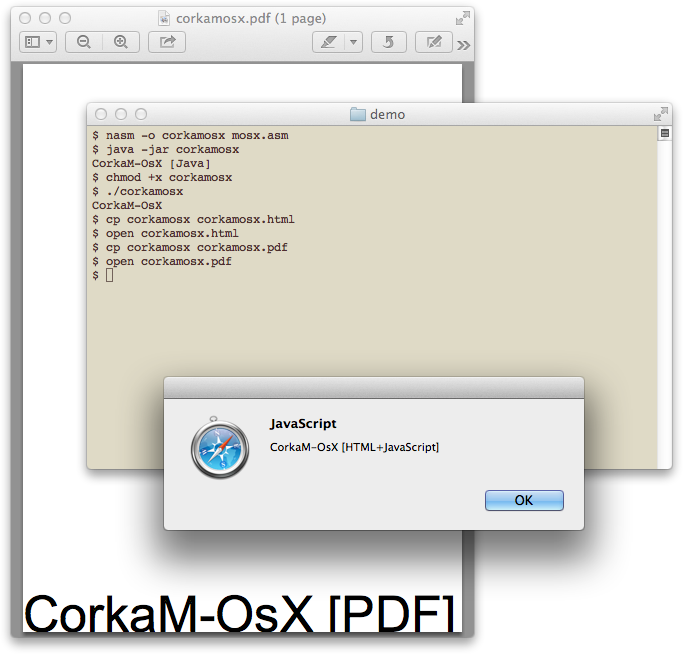
\includegraphics[width=0.7\textwidth]{albertini/img/corkamosx}
  \caption{Un polyglotte binaire sous Mac OS X.}
  \label{fig:albertini:corkamosx}
\end{figure}


\subsection{comparaison d'autres visionneuses \PDF répandues}

Bien que le standard \PDF soit publiquement défini, chaque visionneuse tolère des malformations particulières.

Ceci peut être exploité pour créer un document qui contient un code malveillant qui ne sera vu et traité que par une visionneuse spécifique.

En examinant des visionneuses standards telles que {\em Sumatra}, {\em Chrome} et {\em Adobe Reader}, on s'aperçoit qu'il est possible de faire un document, qui, bien que fonctionnant sans problème sous les trois, se révèle en fait être composé de trois documents indépendants fusionnés, dont chaque élément co-existe en s'ignorant (cf figures~\ref{fig:albertini:pdf-pdf_standardmerged}~et~\ref{fig:albertini:pdf-standard}).

\begin{figure}[ht]
  \centering
  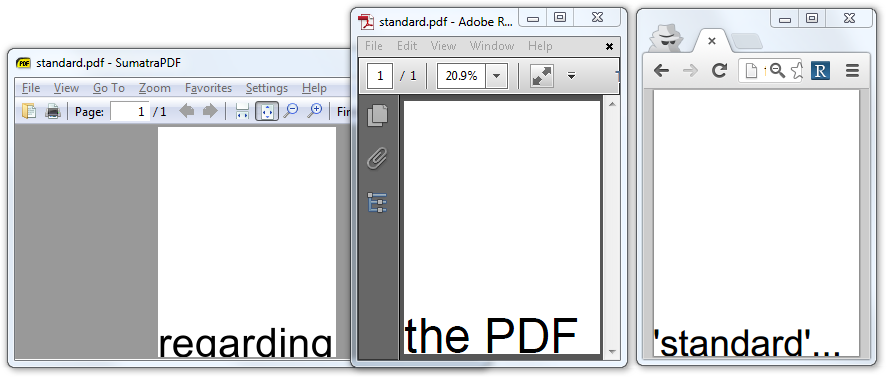
\includegraphics[width=0.8\textwidth]{albertini/img/pdf_standardmerged}
  \caption{Un document interprété différemment par 3 visionneuses distinctes.}
  \label{fig:albertini:pdf-pdf_standardmerged}
\end{figure}

Chaque élément spécifique à une visionneuse étant ignoré par les autres, on peut donc le mutiler au maximum, ce qui fait qu'il pourrait être perçu comme corrompu, et ainsi passer outre des filtres de sécurité: la figure~\ref{fig:albertini:pdf-standard} met en valeur les différences de chaque élement, et ainsi les largesses de chaque visionneuse par rapport aux autres.

\begin{figure}[ht]
  \centering
  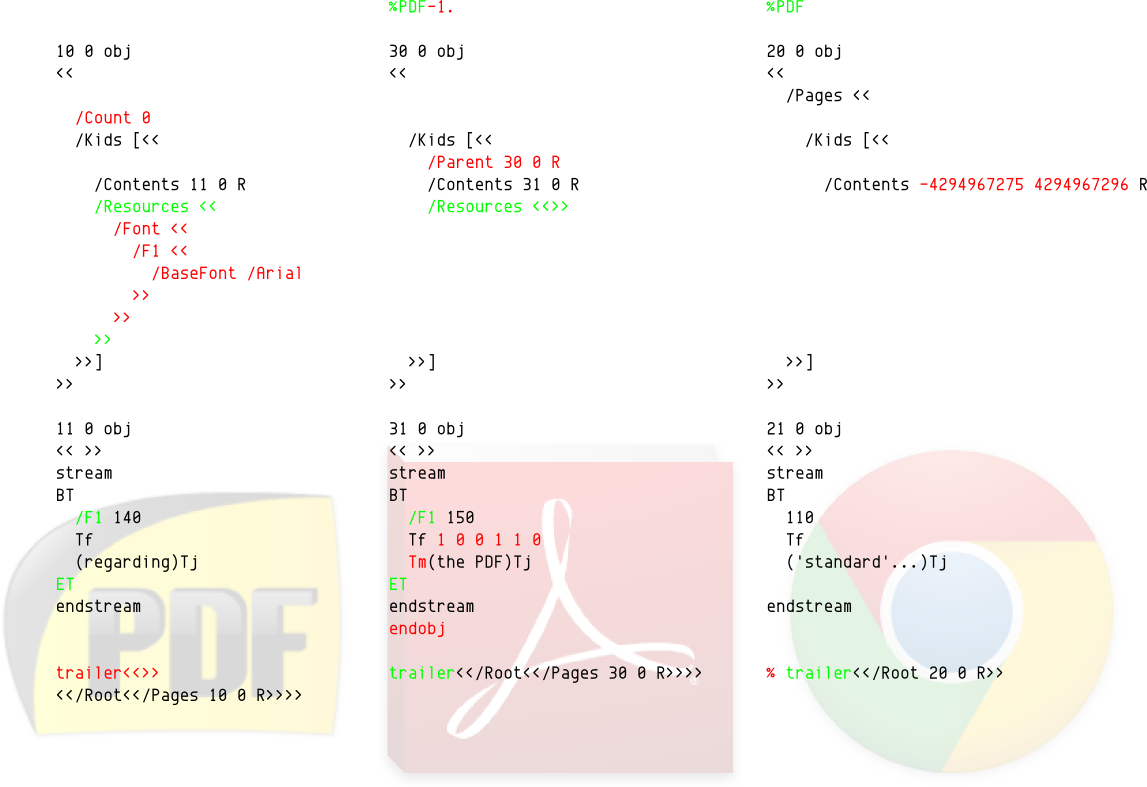
\includegraphics[width=0.8\textwidth]{albertini/img/pdf-standard}
  \caption{Comparaison des différences possibles entre 3 visionneuses.}
  \label{fig:albertini:pdf-standard}
\end{figure}

La visionneuse {\em PDF.JS} est un cas à part: elle bien plus stricte que toutes les autres. Notamment, elle impose~:

\begin{itemize}
\item une table de références \texttt{xref}.
\item une longueur déclarée à chaque \texttt{stream}.
\end{itemize}

qui sont des éléments dont l'absence est tolérée par toutes les autres.

\section{Conséquences pour la sécurité}
Tels des marques de lessive, les outils de sécurité sont comparés selon de trop simples critères: vitesse d'analyse et taux de détection d'un même ensemble empirique de fichiers.

Tout outil d'analyse commercial grand public a donc la lourde responsabilité de ne pas trop s'attarder sur un fichier particulier. En conséquence, il est crucial que le moteur de celui-ci détecte au plus tôt, et efficacement, le type du fichier analysé.

On peut donc imaginer le début de l'exécution d'un tel outil comme une grosse gare de triage: il n'est donc pas surprenant qu'un fichier, une fois détecté comme correspondant à un format connu (comme le montre la figure \ref{fig:albertini:corkamix-vt}), sera analysé comme tel, et donc ne sera pas réanalysé par la suite comme étant d'un autre format.

\begin{figure}[ht]
  \centering
  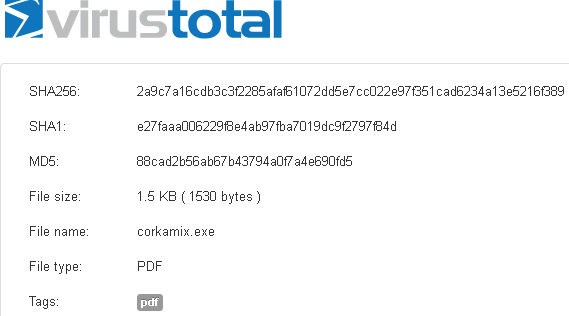
\includegraphics[width=0.8\textwidth]{albertini/img/corkamix-vt}
  \caption{Un exécutable identifié uniquement comme \PDF.}
  \label{fig:albertini:corkamix-vt}
\end{figure}

Quand bien même il le serait, l'outil ne va pouvoir se permettre de réanalyser totalement le fichier comme étant d'un autre format, car il va au bout d'un moment couper l'analyse, pour ne pas s'attarder trop longtemps sur un seul fichier.

Soit la machine qui traite le fichier passe beaucoup de temps (déni de service sur l'anti-virus, ou du moins perte de qualité en matière de vitesse aux yeux des magazines informatiques, ce qui est hors de question pour un produit commercial),
soit l'anti-virus jette un fichier qu'il ne peut analyser de manière exhaustive (déni de service sur la passerelle de fichiers, qui est généralement jugé inacceptable).

Une première démarche pour l'auteur de virus est donc de légitimement feindre un format de fichier: l'outil de sécurité analysera ce fichier comme tel, puis, ne trouvant rien de malveillant dans ce format particulier, déclarera le fichier comme sain.
Ça peut donc se faire simplement en commençant un fichier par la signature \PE,
puis en continuant le fichier comme un fichier \HTML ou \PDF.

De plus, certains outils utilisent un système de cache pour savoir s'ils ont déjà analysé un fichier. Donc, la réutilisation du même fichier --- même sous un autre format --- sautera toute nouvelle analyse via une interception dynamique lors de l'exécution.

Puisqu'un outil de sécurité se doit d'être le plus rapide possible et le plus simple possible, il ne rend comme verdict qu'un booléen, sans tenir compte du format possible du fichier: un booléen par fichier, et non par type possible de fichier.
Le vrai problème, c'est qu'un autre logiciel vulnérable, tel que \JAVA, une visionneuse \PDF ou un navigateur, va peut-être interpréter ce fichier de manière différente.


Une deuxième démarche consiste à inclure un maximum de format, pour que, quelque soit l'ordre d'analyse de l'outil, il atteigne sa limite imposée de temps/cycles, et ainsi qu'il abandonne avant d'avoir pu déterminer si le fichier est sain ou non.

Une autre possibilité est que le fichier cause des problèmes au moteur de l'outil, et qu'il échoue directement.

La première priorité pour un outil de sécurité est de déterminer au plus tôt qu'il y a une combinaison inhabituelle de formats binaires dans un seul fichier, ce qui augmente la suspicion. Si cette combinaison ne concerne aucun cas légitime, tels qu'un \HTML combiné à un exécutable \PE, le fichier peut être classé comme malveillant selon cet unique critère. Malheureusement, cette combinaison de formats peut être perçue comme un avantage technique par des développeurs peu renseignés, et, bien que déconseillée en pratique, peut être rencontrée dans la nature.

D'autre part, tous les navigateurs modernes analysent l'intégralité d'un fichier pour son contenu Web, même s'il est hors norme: par exemple, un fichier constitué d'un exécutable \PE de 27~Mo suivi d'une page Web fonctionnera toujours dans les 2 formats. Un outil de sécurité grand public se devra de se limiter {\it a priori} aux premiers méga-octets, pour optimiser sa performance.

\begin{figure}[ht]
  \centering
  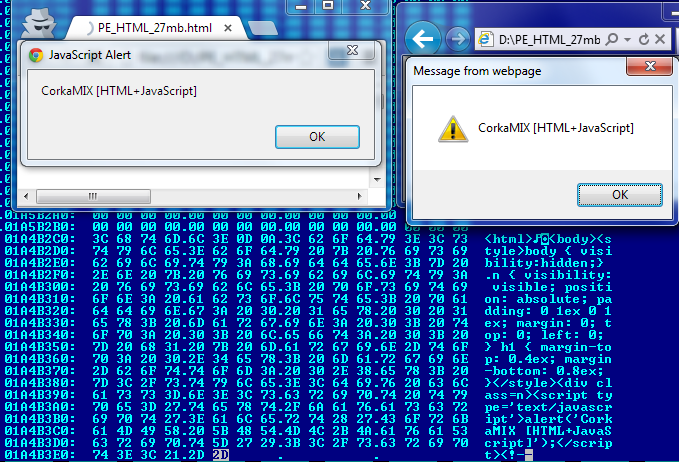
\includegraphics[width=0.8\textwidth]{albertini/img/PE_HTML_27mb}
  \caption{Une page \HTML à la suite d'un \PE de 27Mo.}
  \label{fig:albertini:PE_HTML_27mb}
\end{figure}


\section{Conclusion}

Bien que la plupart excluent d'être combinés à d'autres, certains formats de fichiers autorisent des largesses, ce qui rend la combinaison de formats binaires dans un seul fichier possible.

Ceci a des conséquences de sécurité importantes liées à la confusion entre formats: exécution de virus via les navigateurs, exfiltration de fichier, abandon de l'analyse par les outils de sécurité, menant à considérer un fichier malveillant comme sain (de plus, les malformations possibles de ces formats compliquent l'analyse automatisée et manuelle de virus).

Il semble donc indispensable de ne créer que des standards déterminés par une signature unique au début du fichier.

\emph{Adobe Reader} rejette d'ailleurs, depuis la version 10.1.5 de janvier 2013, tout fichier \PDF commençant par une signature connue telle que \PE, \emph{PNG}, \emph{JPG} \ldots Il ne devrait pourtant en théorie n'accepter que les \PDF commençant par une signature \PDF, mais ce n'est souvent pas le cas dans la pratique.

Les autres visionneuses (\emph{Chrome}, \emph{Sumatra}, \emph{Evince}) acceptent toujours n'importe quel début de fichier. En particulier, \emph{Sumatra} est devenu récemment (version 2.2) plus laxiste en tolérant l'absence de \texttt{endobj} après \texttt{endstream}, alors qu'\emph{Adobe Reader}, au contraire, et comme on s'y attend, renforce progressivement les contrôles de la structure du document.

Une autre possibilité serait d'imposer au système le type de fichier: quand un fichier est téléchargé, il est étiqueté comme son type original, et ensuite le système impose son type, tant qu'une opération externe de dévérouillage de type n'a pas été effectuée.

De même, l'exécution d'un fichier via les APIs \WIN n'impose aucune extension, ce qui rend les exécutables --- pourtant omniprésents dans les virus --- plus facile à lancer, alors qu'il n'y a pas de raison fondamentale qu'on accepte de lancer comme un \PE un document \PDF ou une page \HTML.

\bibliography{albertini/biblio}

%%% Local Variables:
%%% mode: TeX-PDF
%%% TeX-master: "master"
%%% End:


\settitle[CorkaMIX]{Polyglottes binaires et implications}

\newcommand{\TODO}[1]{}
%\newcommand{\TODO}[1]{\textcolor{red}{TODO:~#1}}

\newcommand{\WIN}[0]{\emph{Windows}\xspace}

\newcommand{\ZIP}[0]{\emph{ZIP}\xspace}
\newcommand{\JAVA}[0]{\emph{Java}\xspace}
\newcommand{\GIF}[0]{\emph{GIF}\xspace}
\newcommand{\PE}[0]{\emph{PE}\xspace}
\newcommand{\ELF}[0]{\emph{ELF}\xspace}
\newcommand{\MACHO}[0]{\emph{Mach-O}\xspace}
\newcommand{\JAR}[0]{\emph{JAR}\xspace}
\newcommand{\HTML}[0]{\emph{HTML}\xspace}
\newcommand{\PDF}[0]{\emph{PDF}\xspace}

\setauthor[Ange~Albertini]{Ange Albertini\\
  \email{ange.albertini@gmail.com}}
\institute{Corkami.com}


\maketitle

\begin{abstract}
De l'exploitation à l'infection, les {\it malwares} modernes utilisent de nombreux formats de fichier binaires.
Il est crucial de pouvoir correctement les identifier et les analyser, si possible de manière automatique.
Bien que ces formats soient a priori clairement différenciés, il est parfois possible de combiner certains d'entre eux dans un seul et même fichier.
On parle alors de fichiers {\it polyglottes}.
De tels fichiers {\it polyglottes} ont donc dans un premier temps été créés.
Ensuite, plusieurs caractéristiques non documentées de chaque format concerné ont été rajoutées, pour mettre en évidence l'importance du problème entre les limites des documentations officielles, et la réalité (du monde des virus).
Les conséquences sur le fonctionnement des outils de sécurité sont finalement mises en évidence, avec ce que ça implique pour l'utilisateur final.
\end{abstract}


\section{Introduction}

\subsection{État de l'art}

Un fichier polyglotte est un fichier qui peut être interprété dans plusieurs langages différents.  Un des plus simple d'entre eux, représenté par le Polyglot de David Kendall dans le listing~\ref{lst:albertini:polyglot}, fonctionne en Ruby, Perl, PHP, ksh, Scheme, Lisp, Clojure, Plan. Les {\it polyglottes} peuvent aller beaucoup plus loin, jouant sur les différences d'interprétation et de {\it pré-processing} de chaque langage inclus dans le fichier.


\begin{lstlisting}[language={},caption={Un programme polyglotte simple.},label={lst:albertini:polyglot}]
 (print "Hello, world!\n");
\end{lstlisting}

La première utilisation de fichiers polyglottes dans le monde des virus est GIFAR~\cite{albertini:wikipedia:gifar}~:

un GIFAR résulte de l'ajout d'une classe \JAVA stockée au format \JAR à la suite d'une image au format \GIF. En effet, le \GIF est un format d'image couramment utilisé sur le Web, notamment pour les avatars dans les forums de discussion. Une fois le fichier sur le serveur, il est ensuite utilisable aussi comme une classe \JAVA. Si on utilise cette classe dans un script quelconque sur le serveur, le navigateur laissera accèder à la classe, même si elle est malveillante, car elle est maintenant hébergée sur le même site.

Julia Wolf~\cite{albertini:wolf:omgwtfpdf} a introduit le concept de \ZIP et \emph{Portable Document Format} --- dit \PDF --- combinés, ce qui permet de tromper les outils de sécurité et ainsi permettre d'exfiltrer des informations, ou passer pour un fichier innocent.

Jonas Magazinius~\cite{albertini:magazinius:polyglots} s'est également penché sur la question, en combinant notamment image \emph{JPG} et document \PDF.

En revanche, les formats de fichiers binaires sont, eux, rarement compatibles, car exclusifs: en effet, la majeure partie d'entre eux doivent nécessairement débuter par un marqueur (on parle aussi de \emph{magic number} en anglais), spécifique à chaque format, à de rares exceptions près (tel {\tt 0xcafebabe}, pour le format \MACHO universel et les classes \JAVA).

Il ne semble donc pas possible de combiner des formats binaires en général. Cependant, il y a quelques exceptions:
\begin {itemize}
\item tout d'abord, certains formats de fichier n'ont aucun en-tête, tels que le \emph{Master Boot Record} --- dit \emph{MBR} --- ou les fichiers \emph{COMMAND FILE} --- dit \emph{COM}. Il est donc possible de créer un secteur de démarrage à la fois au format \emph{GRUB} et au format \emph{MBR}~\cite{albertini:scott:metalkiller}, ou bien un fichier \emph{COM} qui soit également un fichier exécutable linux \ELF.

\item d'autre parts, d'autre formats de fichiers n'imposent pas que le marqueur soit présent au début du fichier: c'est le cas des archives (\ZIP, \emph{RAR}\ldots), des pages \HTML, et des documents \PDF.

\item enfin, certains formats, bien que commencant obligatoirement au premier déplacement, autorisent un grand espace entièrement modifiable juste après la signature, tels que le format d'exécutable \emph{Portable Executable} --- dit \PE --- et le format d'image \emph{PICT}.
\end{itemize}

Hélas, certains formats utilisables à des fins malveillantes sont librement combinables dans un seul et même fichier, mais de plus, il s'agit des formats parmi les plus utilisés ces dernières années pour la prolifération de {\it malware}:
en effet, la chaîne d'infection complète par un virus la plus répandue est une page \HTML, contenant du Javascript, qui va charger un fichier \JAVA profitant d'une vulnérabilité, qui lui-même va télécharger le virus final, sous forme d'un exécutable \WIN, au format \emph{PE} --- et on peut effectivement combiner une page \HTML, une classe \JAVA, et un fichier binaire au format \PE.

Un autre vecteur d'infection répandu est un \PDF activant une vulnérabilité, dont le \emph{shellcode} téléchargera un \PE. Et là encore, \PE et \PDF sont combinables dans un seul et même fichier.

\subsection{Pivot}

Le format pivot de la grande majeure partie des virus est le format de binaire universel de \WIN, le format \PE. Pour ce rôle unique dans la chaîne virale, il a donc été choisi comme point de départ.

\section{Exploration du format \PE}
Ce format stipule que le fichier commence par une structure \texttt{IMAGE\_DOS\_HEADER}, de \texttt{0x40} octets:
\begin{itemize}
\item les 2 premiers octets de cette structure définissent un champ appelé \texttt{e\_magic}, qui contient obligatoirement la signature \texttt{MZ}~: Il est donc impossible de le combiner à tout autre format imposant une signature spécifique au déplacement 0.
\item tous les champs suivants, à l'exception du dernier, ne concernent que la fonctionnalité \emph{DOS} de l'exécutable --- qui se borne en majeure partie à afficher un message d'erreur. Elle est totalement ignorée quand le fichier est chargé en tant que \PE.
\item le dernier champ, \texttt{e\_lfanew}, est un pointeur sur 32 bits vers la structure suivante de l'exécutable.
\end{itemize}

On sait donc que notre fichier doit commencer par {\tt M} et {\tt Z}, et qu'au déplacement \texttt{0x3C} doit se trouver un pointeur. Entre les deux, on peut y faire ce que l'on veut, tout en gardant la fonctionalité \PE intacte. On peut même mettre l'en-tête \PE à la fin du fichier sans problème.

\subsection{Création d'une page \HTML dans un exécutable}

Le laxisme omniprésent dans les pages \HTML fait qu'au final, les navigateurs se contentent d'ignorer un peu tout --- quand bien même ce serait de l'information non encodable en \emph{ASCII} --- au cas où un tag \texttt{<HTML>} finirait par être présent.

Ainsi, le simple fait de rajouter à la fin d'un exécutable du code \HTML va en faire une page web fonctionnelle, pour peu qu'on renomme l'extension du fichier, comme le montre la figure~\ref{fig:albertini:htmlnotepad}.

\begin{figure}[ht]
  \centering
  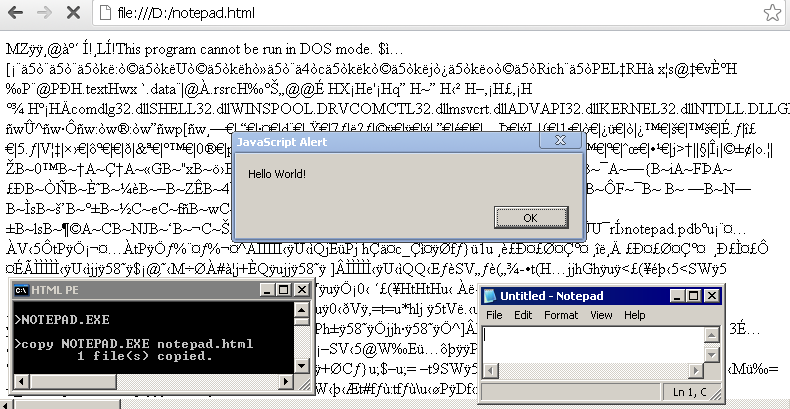
\includegraphics[width=0.8\textwidth]{albertini/img/htmlnotepad}
  \caption{Le bloc-note \WIN avec une page HTML ajoutée à la fin.}
  \label{fig:albertini:htmlnotepad}
\end{figure}

Cela dit, bien que le fichier soit fonctionnel dans les deux formats, les données binaires perturbent l'affichage de la page web, bien que celles-ci soient placées avant le tag ouvrant \texttt{<HTML>}.
On va donc jouer sur les \emph{Cascaded Style Sheet} pour effacer ces données et ainsi avoir un résultat visuellement parfait. Ou sinon, on peut insérer ce tag juste après la signature du \PE, auquel cas on aura juste un \texttt{MZ} affiché sur la page.

De même, si on souhaite rajouter quelque chose après la page web et son script, il nous suffit d'ouvrir un bloc de commentaire non fermé \texttt{<!----}.

À noter que si une page web doit avoir une extension précise pour être visualisée correctement, un exécutable \WIN n'a besoin d'aucune extension particulière pour être exécuté via les APIs \WIN.

\subsection{Concaténation d'un \PDF et d'un exécutable}

La spécification officielle stipule que la première ligne d'un \PDF doit être sa signature:
\begin{center}
  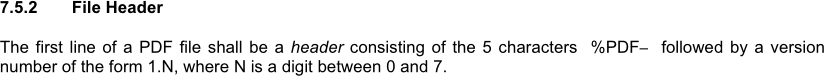
\includegraphics[width=0.8\textwidth]{albertini/img/pdfsigtheory}
\end{center}

En pratique, il n'en n'est rien, il est juste requis sous \emph{Adobe Reader} qu'une signature valide soit présente dans les 1024 (\texttt{0x400}) premiers octets.

\begin{figure}[ht]
  \centering
  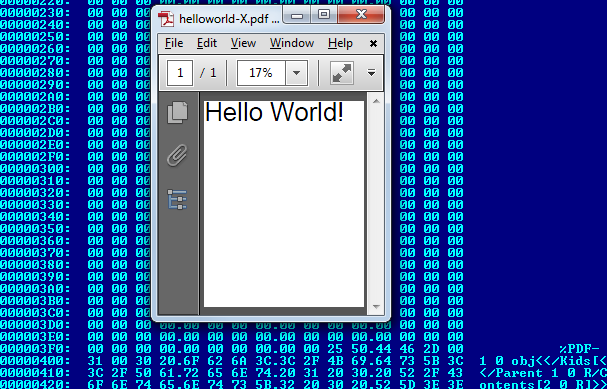
\includegraphics[width=0.8\textwidth]{albertini/img/pdfsigpractice}
  \caption{Un \PDF dont la signature est à la fin des \texttt{1024} premiers octets est toujours reconnu par \emph{Adobe Reader}.}
  \label{fig:albertini:pdfsigpractice}
\end{figure}

On peut donc, dans un premier temps, rajouter à la fin d'un petit exécutable un \PDF dans son intégralité, et les deux fonctionneront encore comme on s'y attend, comme dans la figure~\ref{fig:albertini:tinyPEPDF}.

\begin{figure}[ht]
  \centering
  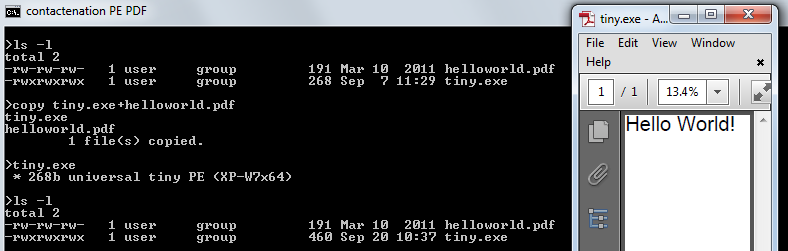
\includegraphics[width=0.8\textwidth]{albertini/img/tinyPEPDF}
  \caption{Un \PDF greffé à la fin d'un petit exécutable \PE.}
  \label{fig:albertini:tinyPEPDF}
\end{figure}

Dans le cas d'un \PE plus gros que \texttt{1024} octets, on devra rajouter la signature \PDF dans l'en-tête \PE.

Il arrive cependant que le \PE, stocké au format binaire, contienne des séquences de caractères qui seront interprétées par la visionneuse \PDF. Pour cela, il suffit d'entourer le reste du \PE d'une structure d'objet \emph{stream} fictive, et ainsi son contenu ne sera pas analysé, puisqu'il n'est pas référencé dans la hiérarchie du document, comme dans la figure~\ref{fig:albertini:pdfnotepad}.

\begin{figure}[ht]
  \centering
  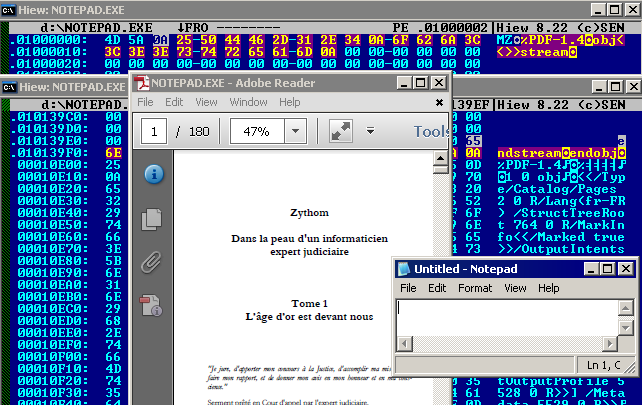
\includegraphics[width=0.8\textwidth]{albertini/img/pdfnotepad}
  \caption{Le bloc-note \WIN avec un fichier \PDF ajouté à la fin.}
  \label{fig:albertini:pdfnotepad}
\end{figure}


\subsection{Une archive \ZIP dans un exécutable}
Le format \ZIP n'impose rien quant au début du fichier --- il est lu en partant de la fin, et tolère des données avant ou après la structure du format elle-même. Un fichier \ZIP peut donc se trouver n'importe où dans un autre fichier.

Une classe \JAVA peut être exécutée directement, ou en étant contenue dans un fichier {\em Java Archive}, dit \JAR.
Un fichier \JAR n'est qu'une archive \ZIP contenant une ou plusieurs classes \JAVA, et un fichier texte (\texttt{manifest}) au contenu bien défini.

Contrairement à un \ZIP standard, un fichier \JAR doit terminer strictement le fichier: si on rajoute ne serait-ce qu'un seul octet à la suite, \JAVA ne reconnaît plus ce fichier comme valide.

\subsection{Récapitulons}

À l'aide des manipulations décrites précédemment, nous obtenons donc:
\begin{enumerate}
\item le début d'un \PE
\item une signature \PDF dans ses \texttt{1024 - 6} premier octets
\item la suite du \PE, inclue dans un objet \texttt{stream} \PDF
\item dans un ordre quelconque~:
\begin{itemize}
\item le reste du \PDF, finissant l'objet fictif
\item la page \HTML
\end{itemize}
\item un \ZIP, optionnellement un \JAR
\end{enumerate}

\section{Détails de mise en oeuvre}

Un simple fichier polyglotte est donc faisable via des opérations de concaténations et quelques modifications manuelles.

Pour pousser l'expérience quant au comportements d'outils de sécurité, des propriétés anormales seront ajoutées aux formats inclus, dans le but de tester leur robustesse.

Afin d'y arriver, l'intégralité du fichier sera faite à la main, pour en garder le contrôle complet.

Toutes les structures sont crées à partir de zéro, en assembleur: en effet, un assembleur standard a la possibilité de définir chaque octet manuellement, et aussi de créer des fonctions et des structures, qui vont faciliter la création du fichier, tout en gardant le contrôle de chaque octet.

Quand un fichier est stocké dans une archive \ZIP sans compression, il est stocké dans son intégralité, à l'identique: inclure un fichier dans une archive ne revient donc qu'à ajouter en-tête et pied de page.

\subsection{Un \PE fait main}

\subsubsection*{Peu d'éléments définis}

Notre exécutable contient \texttt{Hello World} compilé en assembleur standard, mais seulement 18 éléments sont absolument indispensables, toutes structures confondues, tel que le montre la figure~\ref{fig:albertini:empty_pe_header}.

\begin{figure}[ht]
  \centering
  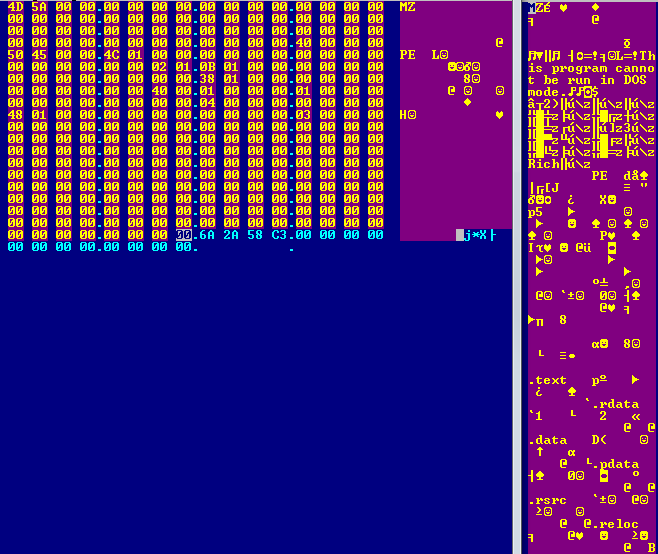
\includegraphics[width=0.8\textwidth]{albertini/img/empty_pe_header}
  \caption{Comparaison d'en-têtes \PE.}
  \label{fig:albertini:empty_pe_header}
\end{figure}

On obtient donc un \PE qui va faire échouer les outils naïfs qui déterminent la validité du fichier d'après des éléments non indispensables.

\subsubsection*{Pas de sections}

Quand un exécutable utilise des alignements faibles, tout l'exécutable est chargé en mémoire indépendamment de la table des sections. Il devient dans ce cas possible de ne définir aucune section (\emph{NumberOfSections = 0}), et de ne pas avoir de table de section (\emph{SizeOfOptionalHeader = 0}).

Là encore, il fera échouer les outils qui analysent ce format section par section.

\subsubsection*{Utilisation d'instructions non documentées}

Un outil de sécurité avancé va essayer d'émuler l'exécution du début du fichier, pour déterminer s'il est malveillant ou non.

Certaines instructions, non documentées, peuvent amener un tel émulateur à abandonner, car il ne peut déterminer comment procéder. La présence de telles instructions ne peut vraisemblablement pas amener à qualifier le fichier de malveillant, car il pourrait s'agir de nouvelles instructions d'un processeur récent.

Certaines de ces instructions comme {\tt SetALC} ou les {\tt nop} multi-octets sont absentes de la documentation Intel (figures~\ref{fig:albertini:undoc_setalc} et \ref{fig:albertini:undoc_nop}), mais présentes dans la documentation AMD (figures~\ref{fig:albertini:salc_amd} et \ref{fig:albertini:nop_amd}), parfois uniquement sous le status \emph{réservé}.


Ces instructions ne sont reconnues dans aucun outil Microsoft (figure~\ref{fig:albertini:corkamix_windbg}), car ils suivent la documentation Intel à la lettre.


\begin{figure}[ht]
  \centering
  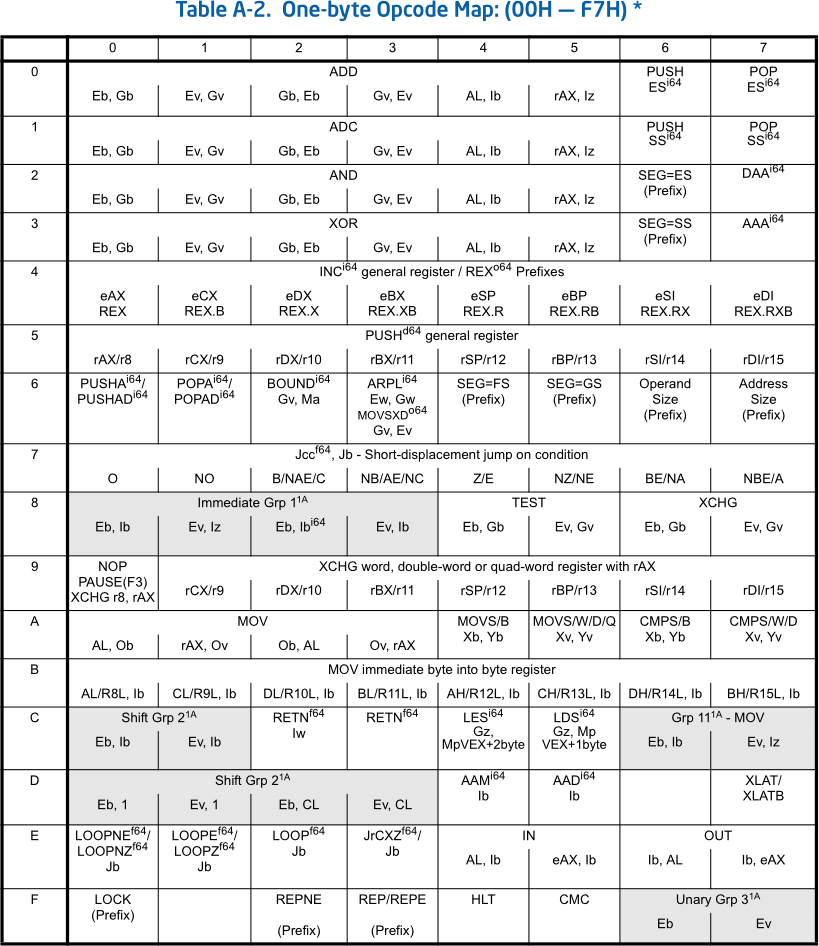
\includegraphics[width=0.8\textwidth]{albertini/img/undoc_setalc}
  \caption{La documentation officielle n'indique rien pour l'octet \texttt{D6}.}
  \label{fig:albertini:undoc_setalc}
\end{figure}

\begin{figure}[ht]
  \centering
  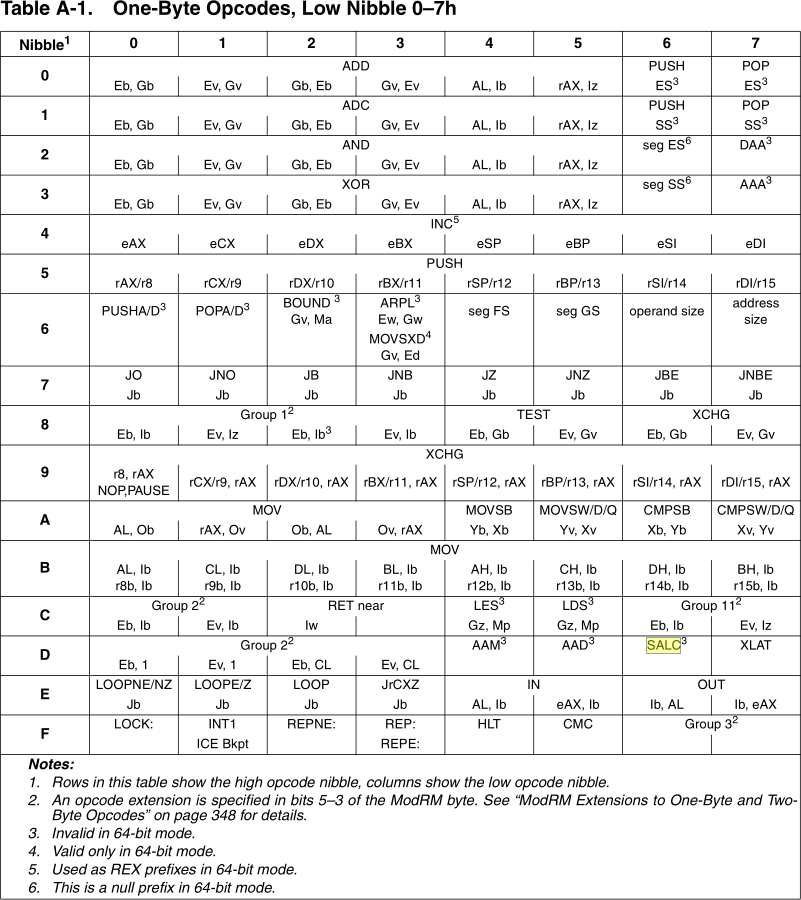
\includegraphics[width=0.8\textwidth]{albertini/img/salc_amd}
  \caption{SetALC est documenté par AMD.}
  \label{fig:albertini:salc_amd}
\end{figure}

\begin{figure}[ht]
  \centering
  \includegraphics[width=0.8\textwidth]{albertini/img/undoc_nop}
  \caption{La documentation Intel ne mentionne NOP que pour les octets \texttt{0F 1F}.}
  \label{fig:albertini:undoc_nop}
\end{figure}

\begin{figure}[ht]
  \centering
  \includegraphics[width=0.8\textwidth]{albertini/img/nop_amd}
  \caption{Le NOP de plusieurs octets est complètement documenté par AMD.}
  \label{fig:albertini:nop_amd}
\end{figure}

\begin{figure}[p]
  \centering
  \includegraphics[width=0.8\textwidth]{albertini/img/corkamix_windbg}
  \caption{WinDbg montre plusieurs instructions inconnues.}
  \label{fig:albertini:corkamix_windbg}
\end{figure}

Pour implémenter ces instructions, on doit générer certaines à la main, un assembleur standard ne les gérant pas forcément.

\subsubsection*{Une structure d'import très compacte}

le \emph{DataDirectory} des imports pointe vers une liste de \emph{descripteurs}.
Cette liste se termine en théorie par un descripteur entièrement nul, mais en réalité uniquement si ses champs \texttt{Name} ou \texttt{FirstThunk} sont nuls.

La table des adresses, si elle est suffisamment petite, peut-être intégrée dans un des descripteurs, alors qu'elle utilise habituellement son propre espace du fichier.

De même, le nom de la DLL, même amputé de son extension, peut être inclus dans un des descripteurs, ainsi que la structure \texttt{IMAGE\_IMPORT\_BY\_NAME} de l'import, alors qu'eux aussi sont censés être instanciés séparément, hors des descripteurs.

On obtient donc une table d'import très compacte, avec beaucoup d'irrégularités, mais pourtant 100~\% gérée et fonctionnelle (figure~\ref{fig:albertini:imports}) par \WIN.

\begin{figure}[p]
  \centering
  \includegraphics[width=0.5\textwidth]{albertini/img/imports}
  \caption{Une structure d'imports avec beaucoup de malformations.}
  \label{fig:albertini:imports}
\end{figure}

Ces astuces font que les outils les plus avancés échouent à analyser le \PE parfaitement. Notamment, à l'heure de création de ces recherches, la dernière version de Hiew et IDA échouent à les gérer (figure~\ref{fig:albertini:imports_error}).

\begin{figure}[p]
  \centering
  \includegraphics[width=0.5\textwidth]{albertini/img/imports_error}
  \caption{Une structure d'imports non gérée par Hiew ou IDA.}
  \label{fig:albertini:imports_error}
\end{figure}



\subsection{Un \PDF très compact}
La signature \PDF, bien qu'officiellement \texttt{\%PDF-1.?}, peut en fait être tronquée, selon la visionneuse employée.

La signature de fin \texttt{\%\%EOF} est absolument superflue, ansi que toute référence à une longueur dans les objets \texttt{stream}.

De même, la table \texttt{xref} est supprimable, ansi que les terminateurs d'objet \texttt{endobj}.

Enfin, le trailer final est réduit à son strict minimum.

On obtient donc, dans des cas extrêmes, un fichier \PDF particulièrement réduit de 36 octets fonctionnant sous Adobe Reader (listing~\ref{lst:albertini:tinypdf}).

\begin{lstlisting}[language={},caption={Un \PDF valide de 36 octets.},label={lst:albertini:tinypdf}]
%PDF- trailer<</Root<</Pages<<>>>>>>
\end{lstlisting}

\subsection{Un \emph{patchwork} binaire}

Au final, on obtient un fichier fonctionnel dans tous les formats inclus (figure~\ref{fig:albertini:corkamix}), et de nombreuses caractéristiques non documentées, qui font échouer des outils d'analyse et des anti-virus répandus.

\begin{figure}[p]
  \centering
  \includegraphics[width=0.7\textwidth]{albertini/img/corkamix}
  \caption{Un joli \emph{patchwork}}
  \label{fig:albertini:corkamix}
\end{figure}

On peut rajouter de nombreux formats dans le fichier \ZIP lui-même, mais ça ne présente aucun challenge particulier.

Un tel mélange binaire ne nécessite pas de faire ces fichiers à la main: on peut prendre des fichiers tout à fait standards et obtenir un résultat analogue, bien qu'ayant un air plus familier (figure~\ref{fig:albertini:sssticmix}).

\begin{figure}[p]
  \centering
  \includegraphics[width=0.7\textwidth]{albertini/img/sssticmix}
  \caption{Un polyglotte binaire avec un air familier.}
  \label{fig:albertini:sssticmix}
\end{figure}

\subsection{Autres systèmes d'exploitations}

Un esprit moqueur serait tenté de se contenter de blâmer \emph{Microsoft} et \emph{Adobe} pour leur laxisme, et le fait d'accepter ainsi n'importe quel format binaire.

\subsubsection{Linux}

En regardant le format \PDF dans un premier temps, on s'aperçoit que les visionneuses \PDF standards sous Linux, bien que n'acceptant pas le \PDF particulier généré précedemment, n'en sont pas pour autant vraiment rigoureuses.

En effet, en creusant un peu, on s'aperçoit que de nombreux outils \PDF tels qu'Evince ou la visionneuse standard d'Ubuntu, acceptent un \PDF ne contenant même pas de signature \texttt{\%PDF} --- même partielle --- ce qu'\emph{Adobe Reader} refusera immédiatement.

Le format binaire Linux, {\it Executable File Format} --- dit \ELF --- n'impose rien de particulier concernant le fichier lui-même. Créer un tel polyglotte basé sur un \ELF plutôt qu'un \PE ne présente alors pas de difficulté particulière, tel que le montre la figure \ref{fig:albertini:corkaminux}.

\begin{figure}[p]
  \centering
  \includegraphics[width=0.7\textwidth]{albertini/img/corkaminux}
  \caption{Un polyglotte binaire sous Linux.}
  \label{fig:albertini:corkaminux}
\end{figure}


\subsubsection{Mac OS X}

Les visionneuses \PDF standards Mac OS X et iOS sont elles, beaucoup plus strictes.

Elles refusent toute signature incomplète ou absente. Les seules malformations théoriques acceptées sont l'absence de \texttt{xref}, longueurs de flux (\texttt{stream /length}), et signature de fin de fichier \texttt{\%\%EOF}.

Le format binaire de Mac OS X, le \MACHO (pour \emph{Mach Object}) ne présente, à l'instar des formats \PE et \ELF, aucune difficulté particulière une fois qu'on a la maîtrise de leur structure binaire (figure~\ref{fig:albertini:corkamosx}).
\begin{figure}[p]
  \centering
  \includegraphics[width=0.7\textwidth]{albertini/img/corkamosx}
  \caption{Un polyglotte binaire sous Mac OS X.}
  \label{fig:albertini:corkamosx}
\end{figure}


\subsection{comparaison d'autres visionneuses \PDF répandues}

Bien que le standard \PDF soit publiquement défini, chaque visionneuse tolère des malformations particulières.

Ceci peut être exploité pour créer un document qui contient un code malveillant qui ne sera vu et traité que par une visionneuse spécifique.

En examinant des visionneuses standards telles que {\em Sumatra}, {\em Chrome} et {\em Adobe Reader}, on s'aperçoit qu'il est possible de faire un document, qui, bien que fonctionnant sans problème sous les trois, se révèle en fait être composé de trois documents indépendants fusionnés, dont chaque élément co-existe en s'ignorant (cf figures~\ref{fig:albertini:pdf-pdf_standardmerged}~et~\ref{fig:albertini:pdf-standard}).

\begin{figure}[ht]
  \centering
  \includegraphics[width=0.8\textwidth]{albertini/img/pdf_standardmerged}
  \caption{Un document interprété différemment par 3 visionneuses distinctes.}
  \label{fig:albertini:pdf-pdf_standardmerged}
\end{figure}

Chaque élément spécifique à une visionneuse étant ignoré par les autres, on peut donc le mutiler au maximum, ce qui fait qu'il pourrait être perçu comme corrompu, et ainsi passer outre des filtres de sécurité: la figure~\ref{fig:albertini:pdf-standard} met en valeur les différences de chaque élement, et ainsi les largesses de chaque visionneuse par rapport aux autres.

\begin{figure}[ht]
  \centering
  \includegraphics[width=0.8\textwidth]{albertini/img/pdf-standard}
  \caption{Comparaison des différences possibles entre 3 visionneuses.}
  \label{fig:albertini:pdf-standard}
\end{figure}

La visionneuse {\em PDF.JS} est un cas à part: elle bien plus stricte que toutes les autres. Notamment, elle impose~:

\begin{itemize}
\item une table de références \texttt{xref}.
\item une longueur déclarée à chaque \texttt{stream}.
\end{itemize}

qui sont des éléments dont l'absence est tolérée par toutes les autres.

\section{Conséquences pour la sécurité}
Tels des marques de lessive, les outils de sécurité sont comparés selon de trop simples critères: vitesse d'analyse et taux de détection d'un même ensemble empirique de fichiers.

Tout outil d'analyse commercial grand public a donc la lourde responsabilité de ne pas trop s'attarder sur un fichier particulier. En conséquence, il est crucial que le moteur de celui-ci détecte au plus tôt, et efficacement, le type du fichier analysé.

On peut donc imaginer le début de l'exécution d'un tel outil comme une grosse gare de triage: il n'est donc pas surprenant qu'un fichier, une fois détecté comme correspondant à un format connu (comme le montre la figure \ref{fig:albertini:corkamix-vt}), sera analysé comme tel, et donc ne sera pas réanalysé par la suite comme étant d'un autre format.

\begin{figure}[ht]
  \centering
  \includegraphics[width=0.8\textwidth]{albertini/img/corkamix-vt}
  \caption{Un exécutable identifié uniquement comme \PDF.}
  \label{fig:albertini:corkamix-vt}
\end{figure}

Quand bien même il le serait, l'outil ne va pouvoir se permettre de réanalyser totalement le fichier comme étant d'un autre format, car il va au bout d'un moment couper l'analyse, pour ne pas s'attarder trop longtemps sur un seul fichier.

Soit la machine qui traite le fichier passe beaucoup de temps (déni de service sur l'anti-virus, ou du moins perte de qualité en matière de vitesse aux yeux des magazines informatiques, ce qui est hors de question pour un produit commercial),
soit l'anti-virus jette un fichier qu'il ne peut analyser de manière exhaustive (déni de service sur la passerelle de fichiers, qui est généralement jugé inacceptable).

Une première démarche pour l'auteur de virus est donc de légitimement feindre un format de fichier: l'outil de sécurité analysera ce fichier comme tel, puis, ne trouvant rien de malveillant dans ce format particulier, déclarera le fichier comme sain.
Ça peut donc se faire simplement en commençant un fichier par la signature \PE,
puis en continuant le fichier comme un fichier \HTML ou \PDF.

De plus, certains outils utilisent un système de cache pour savoir s'ils ont déjà analysé un fichier. Donc, la réutilisation du même fichier --- même sous un autre format --- sautera toute nouvelle analyse via une interception dynamique lors de l'exécution.

Puisqu'un outil de sécurité se doit d'être le plus rapide possible et le plus simple possible, il ne rend comme verdict qu'un booléen, sans tenir compte du format possible du fichier: un booléen par fichier, et non par type possible de fichier.
Le vrai problème, c'est qu'un autre logiciel vulnérable, tel que \JAVA, une visionneuse \PDF ou un navigateur, va peut-être interpréter ce fichier de manière différente.


Une deuxième démarche consiste à inclure un maximum de format, pour que, quelque soit l'ordre d'analyse de l'outil, il atteigne sa limite imposée de temps/cycles, et ainsi qu'il abandonne avant d'avoir pu déterminer si le fichier est sain ou non.

Une autre possibilité est que le fichier cause des problèmes au moteur de l'outil, et qu'il échoue directement.

La première priorité pour un outil de sécurité est de déterminer au plus tôt qu'il y a une combinaison inhabituelle de formats binaires dans un seul fichier, ce qui augmente la suspicion. Si cette combinaison ne concerne aucun cas légitime, tels qu'un \HTML combiné à un exécutable \PE, le fichier peut être classé comme malveillant selon cet unique critère. Malheureusement, cette combinaison de formats peut être perçue comme un avantage technique par des développeurs peu renseignés, et, bien que déconseillée en pratique, peut être rencontrée dans la nature.

D'autre part, tous les navigateurs modernes analysent l'intégralité d'un fichier pour son contenu Web, même s'il est hors norme: par exemple, un fichier constitué d'un exécutable \PE de 27~Mo suivi d'une page Web fonctionnera toujours dans les 2 formats. Un outil de sécurité grand public se devra de se limiter {\it a priori} aux premiers méga-octets, pour optimiser sa performance.

\begin{figure}[ht]
  \centering
  \includegraphics[width=0.8\textwidth]{albertini/img/PE_HTML_27mb}
  \caption{Une page \HTML à la suite d'un \PE de 27Mo.}
  \label{fig:albertini:PE_HTML_27mb}
\end{figure}


\section{Conclusion}

Bien que la plupart excluent d'être combinés à d'autres, certains formats de fichiers autorisent des largesses, ce qui rend la combinaison de formats binaires dans un seul fichier possible.

Ceci a des conséquences de sécurité importantes liées à la confusion entre formats: exécution de virus via les navigateurs, exfiltration de fichier, abandon de l'analyse par les outils de sécurité, menant à considérer un fichier malveillant comme sain (de plus, les malformations possibles de ces formats compliquent l'analyse automatisée et manuelle de virus).

Il semble donc indispensable de ne créer que des standards déterminés par une signature unique au début du fichier.

\emph{Adobe Reader} rejette d'ailleurs, depuis la version 10.1.5 de janvier 2013, tout fichier \PDF commençant par une signature connue telle que \PE, \emph{PNG}, \emph{JPG} \ldots Il ne devrait pourtant en théorie n'accepter que les \PDF commençant par une signature \PDF, mais ce n'est souvent pas le cas dans la pratique.

Les autres visionneuses (\emph{Chrome}, \emph{Sumatra}, \emph{Evince}) acceptent toujours n'importe quel début de fichier. En particulier, \emph{Sumatra} est devenu récemment (version 2.2) plus laxiste en tolérant l'absence de \texttt{endobj} après \texttt{endstream}, alors qu'\emph{Adobe Reader}, au contraire, et comme on s'y attend, renforce progressivement les contrôles de la structure du document.

Une autre possibilité serait d'imposer au système le type de fichier: quand un fichier est téléchargé, il est étiqueté comme son type original, et ensuite le système impose son type, tant qu'une opération externe de dévérouillage de type n'a pas été effectuée.

De même, l'exécution d'un fichier via les APIs \WIN n'impose aucune extension, ce qui rend les exécutables --- pourtant omniprésents dans les virus --- plus facile à lancer, alors qu'il n'y a pas de raison fondamentale qu'on accepte de lancer comme un \PE un document \PDF ou une page \HTML.

\bibliography{albertini/biblio}

%%% Local Variables:
%%% mode: TeX-PDF
%%% TeX-master: "master"
%%% End:

\end{document}

%% Publication
%% ===========
%% 
%% Vous devez envoyer les *sources* à actes (AT) lists.sstic.org avant
%% la date butoir.
%% 
%% L'auteur consciencieux prendre soin de corriger tous les warnings
%% avant de nous envoyer ses sources :)
%%
%% Vous pouvez envoyer une archive complète (.tar.gz), ou un patch, ou
%% un lien vers votre repository, etc.
%% 
%%% Local Variables:
%%% mode: TeX-PDF
%%% TeX-master: "master"
%%% End:
